% !TEX root = ../thesis.tex

%
%\begin{figure*}[t]
%	
%	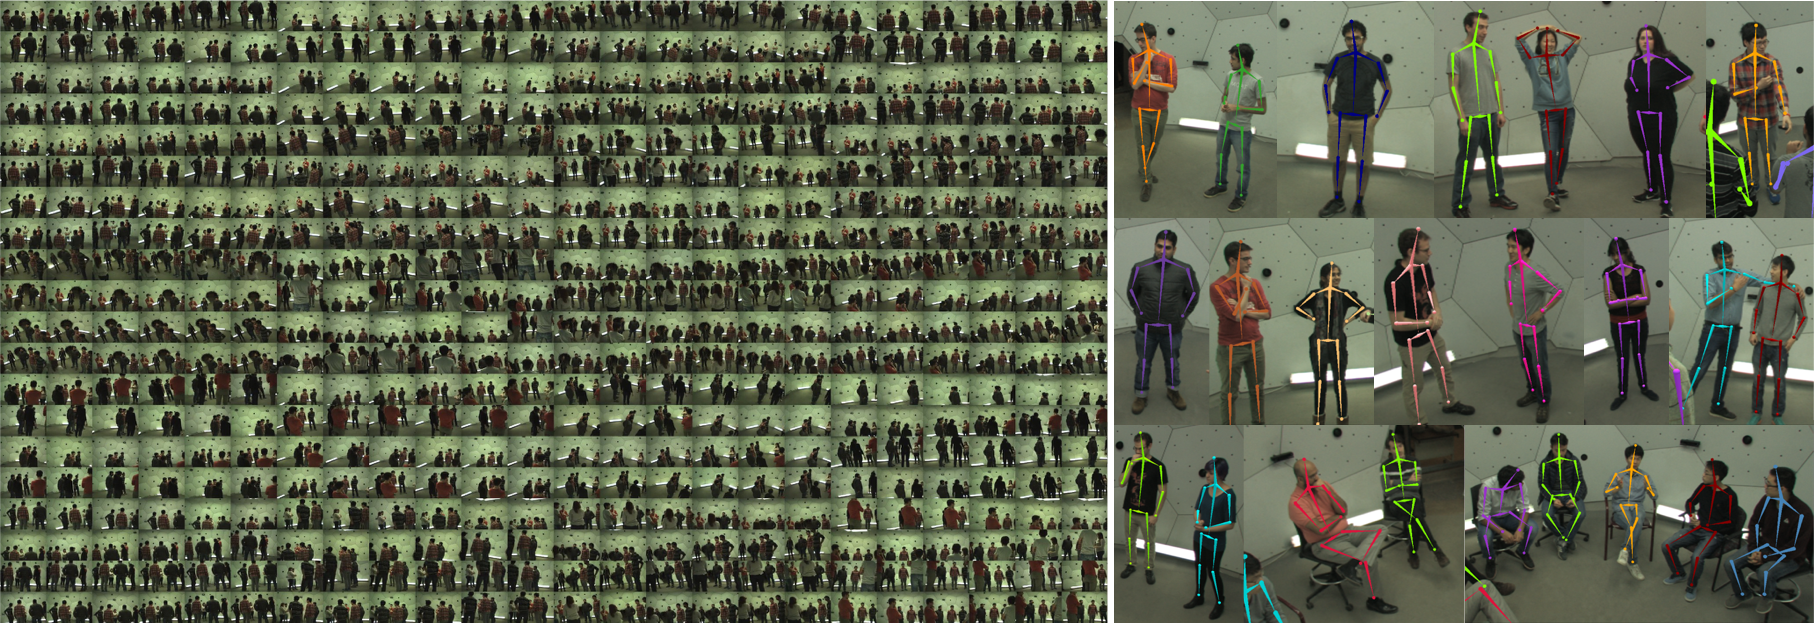
\includegraphics[width=\linewidth]{imgs/Teaser_0814}
%	\caption{(Left) 480 unique VGA views capturing a social interaction within the Panoptic Studio. (Right) HD example views showing frequently occurring postures that carry rich social signals, with 3D body pose automatically annotated by our method.} 
%	\label{fig:iconicPoses}
%\end{figure*}

\chapter{Introduction}
%The way humans communicate is one of the clearest factors that differentiates us from other animals. 
Along with verbal language, we use many other channels for communication, including facial expression, body gestures, hand motions, and interpersonal proximity, collectively referred to as \emph{nonverbal social signals}. The use of all these channels is important in social interactions, where subtle emotions and intentions are transmitted via the combination of such signals~\cite{Moore13}. Endowing machines with such social interaction abilities is an essential goal of Artificial Intelligence (AI) to make machines that can effectively cooperate with humans.% This area is related to multidisciplinary research fields covering psychology, natural language processing, affective computing, human-robot interaction, machine learning, and computer vision.


A way to endow machines with such social skills would be to encode all the rules that humans observe during social communication~\cite{cassell1994animated, cassell2000embodied}. Unfortunately, nonverbal interaction is still poorly understood despite its importance in social communication~\cite{Mehrabian67,Mehrabian81,Birdwhistell-1970}, making it hard to formalize all rules about how to understand and use social signals. An alternative direction of this ``symbolic" paradigm~\cite{newell1976} is to take the ``non-symbolic" (or connectionist) approach~\cite{rumelhart1986parallel} to learn the way humans communicate purely from the data without any hand-coded high level representations. Interestingly, we have recently witnessed significant progress in Natural Language Processing (NLP) showing the potential to allow machines to ``freely'' communicate with humans using written language and speech~\cite{young2018recent}. This success has been led by data-driven approaches leveraging large-scale language datasets and a powerful modeling tool, deep neural networks~\cite{lecun2015deep}, to automatically learn the patterns of human verbal communication. Remarkably, these achievements have not made extensive use of the prior knowledge about grammar and the structure of languages that linguists have accumulated over centuries. Motivated by this, this thesis hypothesizes that a similar approach can be an important breakthrough in modeling nonverbal communication. 

%
%\label{sec:introduction}
%\begin{figure}[h]
%	\centering
%	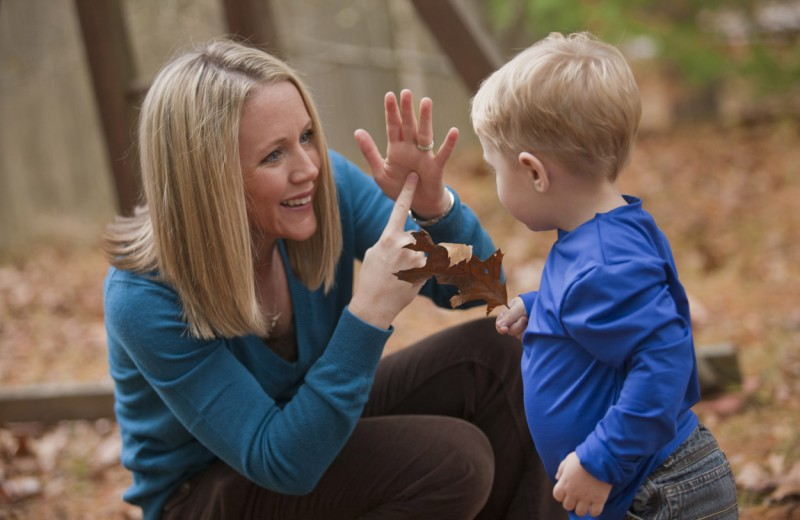
\includegraphics[trim=0 0 0 0, clip=true, height=0.2\columnwidth]{figures/intro_1}
%	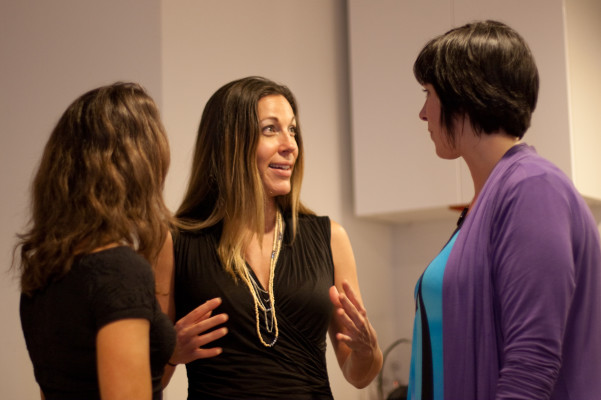
\includegraphics[trim=0 0 0 0, clip=true, height=0.2\columnwidth]{figures/intro_5}
%	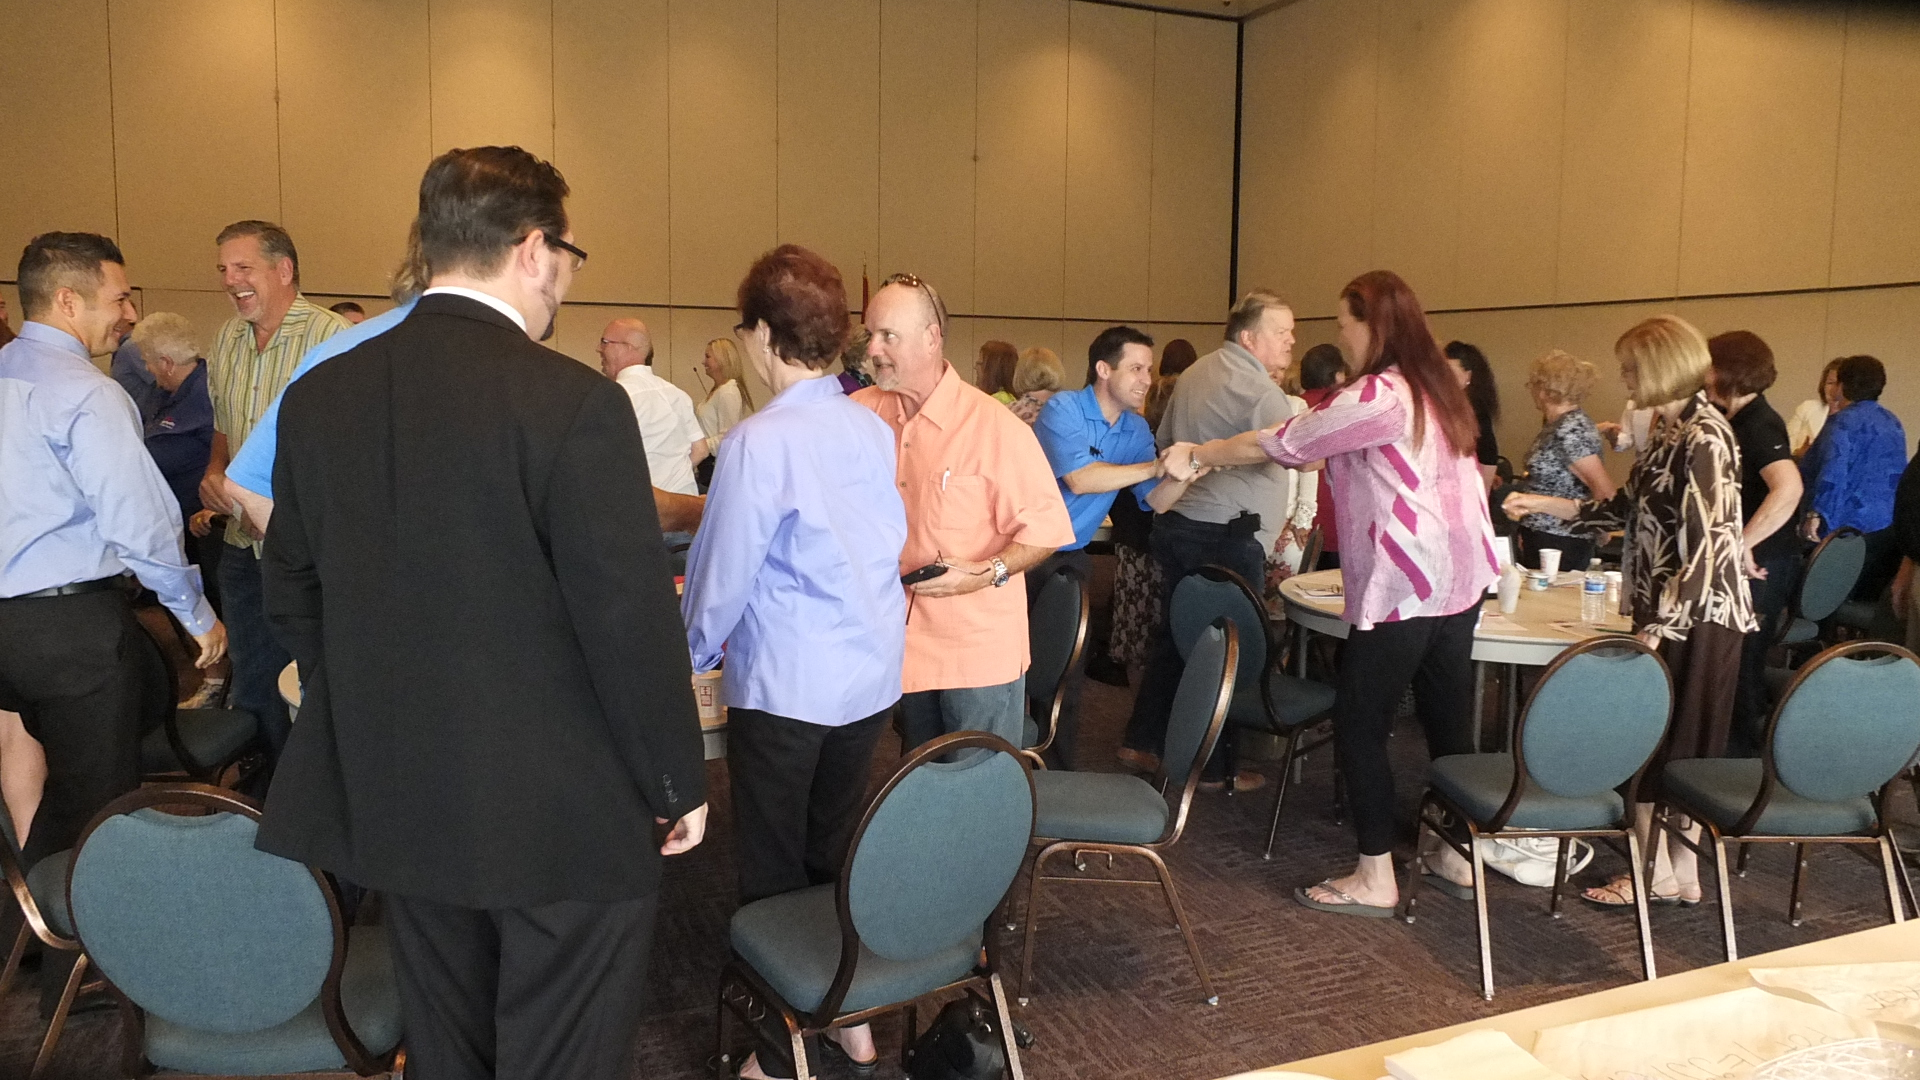
\includegraphics[trim=0 0 0 0, clip=true, height=0.2\columnwidth]{figures/intro_3}
%	\caption{Nonverbal signals play an important role in social communication to transmit messages that cannot be conveyed by verbal language. However, we still lack an understanding of the underlying protocols of these signals. Two major challenges to computationally analyze nonverbal signals in social communication are: (1) measuring the signals at high resolution and (2) modeling nonverbal communication as information flow in the high dimensional space.}	
%	%	\caption{Kinesic signals play important roles in social communication to transmit messages that cannot be conveyed by verbal languages. In this thesis proposal, we present a system and method to measure full body kinesic signals including anatomical landmarks from body, face, and hands. We also propose an approach to model kinesic signals in social interaction by optimizing a prediction function in continuous high bandwidth kinesic signal space.}	
%	\label{fig:ch1_intro}
%\end{figure}


However, there exists a fundamental difficulty in building a data-driven nonverbal communication model: the data is extremely rare. In the verbal language domain, words contain the full expressive power to record verbal signals by a composition of a handful of discrete symbols. Especially on the Internet, there already exist millions of articles or dialogues which are readily usable for data-driven methods (either supervised or unsupervised). However, for nonverbal signals, how to ``record" or collect these signals is uncertain. Imagine a situation where a group of people are communicating in our daily life. The positions and orientations of individuals, their body gestures, gaze, and facial expressions (among others) are the data we are interested in. Notably, these social signals emitted from all people in the group need to be simultaneously sensed to study their correlation and causality. Although there also exist millions of videos where our daily activities---including social interactions---are captured on the Internet, these raw videos cannot be directly used because we have to first measure the behavioral cues (relative location, face, body pose, and so on) from the raw pixels to focus on investigating the rules of nonverbal interactions. %Fortunately, measuring human behavior including person detection~\cite{}, body pose estimation~\cite{}, face keypoint detection, hand keypoint estimation, markerless motion captures have all been greatly advanced, enabling us to collect non-verbal signal dataset.


This thesis explores two scientific questions to computationally study social signals in nonverbal communication: (1) how to measure the ``full spectrum of social signals", including facial expressions, hand gestures, and body motions of an interacting group and (2) how to formalize a ``Connectionist" model by leveraging these new types of signal measurements aiming to teach machines how to decode and encode nonverbal signals to genuinely interact with humans. As major advancements in science are nearly always preceded by innovations in engineering that enable us to measure the world, the first part of this thesis starts by presenting a novel system and method to sense and measure such signals. As a core contribution, a massively multiview capture system, the \emph{Panoptic Studio} shown in the top of Figure~\ref{fig:teaser}, is built to capture naturally interacting multiple people in social situations (Chapter~\ref{chapter:system}). Methods to measure the subtle 3D movements of anatomical landmarks including facial expression, hand gestures, and body motions are also presented, leveraging a large number of views of the Panoptic Studio System (Chapter~\ref{chapter:trajectory}, \ref{chapter:mocap}, and  \ref{chapter:totalcapture}). Our system and method enable us to measure and record the various behavioral cues in face-to-face interactions without using any intrusive devices or artificial markers. 


In the latter part of this thesis, we computationally study the dynamics among interpersonal social signals by leveraging a large-scale social signal corpus built from our system and measurement method. In this research, we verify that the social signals naturally emerging in an interacting group are highly correlated and predictive each other. To achieve the goal, we first collect a large scale dataset where the full spectrum social signals are measured from hundreds of participants in a carefully designed triadic interaction scenario (Chapter~\ref{chapter:dataset}). Then, we formalize a social signal prediction problem as a way to model the dynamics and correlations between various channels of social signals (Chapter~\ref{chapter:prediction}). We explore several social signal prediction tasks defined with various input and output signals to verify the strong links among them. %To this end, we apply the models to build an artificial agent that mimics the nonverbal communication skills of humans, which we refer to as a ``social Artificial Intelligence".

%
%In the latter part of this thesis, we introduce a new research task to build machines that can encode and decode social signals. We hypothesize that the social signals naturally emerging in an interacting group are highly correlated and predictive each other. Thus, we formalize a social signal prediction problem as a way to model such correlation. To demonstrate this, we first collect a large scale dataset where the full spectrum social signals are measured from hundreds of participants in a carefully designed triadic interaction scenario (Chapter~\ref{chapter:dataset}). Then, we leverage this dataset to explore a social signal prediction task to mimic the social behaviors of humans (Chapter~\ref{chapter:prediction}); we formulate that humans are communicating by receiving a set of social signals from others and emitting response signals as output, which are again directed to others as inputs. Machines can learn nonverbal communication skills by automatically finding the patterns between these signal flows. Importantly, our dataset allows us to investigate wide channels of nonverbal cues and their correlations. We explore several subtasks of the social signal prediction to verify the existence of the correlation of social signals, and finally present a framework to build a social Artificial Intelligence by consolidating our social signal prediction modules. 


\section{Key Challenges}
This thesis aims to computationally model social interaction, focusing on nonverbal social signals. Two major challenges in pursuing the direction are addressed.
%To achieve the goal, the signals naturally emerging from interacting people should be obtained first. However, it is challenging to capture and measure such signals in social situations due to multiple challenges addressed in this section. The lack of existing data limits the opportunity to computationally model nonverbal social communication, causing a singular focus on limited measurements and scenarios (e.g., face only~\cite{tronick1989infant} or a table setup allowing limited body motions~\cite{gunes2006bimodal, banziger2012introducing, de2004modeling}). In this thesis, two major challenges in pursuing computational analysis of nonverbal social interactions are addressed.\\ % . 
\paragraph{How To Sense and Measure Nonverbal Social Signals:}
To achieve the goal of this thesis, the signals naturally emerging from interacting people should be obtained first. However, it is challenging to sense and measure such social signals, because of the following three reasons. First, during social interactions, strong occlusions emerge functionally (e.g., people systematically face each other while interacting, bodies are occluded by gesticulating limbs). Thus, measurements from a monocular view can hardly capture the entire social signals of all the people involved in the communication (e.g., Figure~\ref{fig:teaser}). Second, subtle motions from faces and hands that play an important role in social interactions should be measured together with large motions from torsos and limbs. This introduces a sensing challenge because often face and hand motions are captured at close range~\cite{beeler2010high,ghosh2011multiview, Beeler2011, bradley2010high, valgaerts2012lightweight, Oikonomidis-12, Tompson-14a, Sridha-15, Tzionas-16}, while torso and limb motions are captured in a sufficiently large working volume where people can freely move~\cite{deAguiar-2008, Gall-09, Stoll-11, Elhayek-15}. Third, the social signals should be measured non-intrusively to allow the people involved a communication to behave naturally and voluntarily. Thus, popular marker-based motion capture systems (e.g., \cite{VICON}) are not applicable. 

Despite the advances in human sensing and markerless motion capture fields in computer vision and graphics, these challenges have not been fully solved yet. Most of the existing methods prior to this thesis focus on the motion of a single subject~\cite{deAguiar-2008,Vlasic-2009,Furukawa2008,Gall-09, Stoll-11, Baak-13,Shotton-13} or exaggerated motions of actors~\cite{Ye-2012,Liu-2013}. Importantly, there is no existing system that can track, without markers, the human body, face, and hands of multiple individuals simultaneously.

Due the limit of available measurement tools, social signals are studied in limited scenarios, for example: (1) studies only focus on face signals ignoring body motions~\cite{messinger2009automated, lucas_trust_2016,mckeown2012semaine}; (2) studies consider situations in a table setup where participants' motions are limited~\cite{carletta2005ami, Lepri-12,messinger2009automated, nojavanasghari2016emoreact, lucas_trust_2016,mckeown2012semaine}; (3) studies assume a small number of people (mostly dyadic communications)~\cite{messinger2009automated,nojavanasghari2016emoreact, lucas_trust_2016, katsimerou2016crowdsourcing,mckeown2012semaine,gunes2006bimodal}.
% 
%
%are rarely measured in social situations, since most of the face and hand systems assume a close distance to the target which can be hardly used for body motion capture system. It is necessary that such signals from faces and hands are measured together with large motion from torsos and limbs, because subtle messages for communications are usually transmitted by the organized motion of the whole body.\\ 
%
%Second, voluntary motions in a social signals should be captured by a non-intrusive method
%
%Third, large motions and subtle details should be capture together. 
%
% This means that a multiview setup to is needed. 
%
% To accurately analyze social interactions, a volume sufficient to house a social group should be assumed, yet all the subtle details of the motion where important social signals are embedded must be captured. A laboratory setup with multiple cameras is preferred to achieve this objective, and it is expected that the sensing challenges can be reduced according to increasing unique view points. However, in most prior work, a few cameras are often used, and, thus, limited research directions are only considered, for example: (1) studies only focus on face signals ignoring body motions~\cite{messinger2009automated, lucas_trust_2016,mckeown2012semaine}; (2) studies consider situations in a table setup where participants' motions are limited~\cite{carletta2005ami, Lepri-12,messinger2009automated, nojavanasghari2016emoreact, lucas_trust_2016,mckeown2012semaine}; (3) studies assume only few number of people (e.g., dyadic communications)~\cite{messinger2009automated,nojavanasghari2016emoreact, lucas_trust_2016, katsimerou2016crowdsourcing,mckeown2012semaine,gunes2006bimodal}.
%
%%\noindent \textbf{How To Measure Kinesic Signals}:  
%For computational analysis, captured raw data (images or videos) should be semantically labeled. For example, a human can infer 3D structure of other people and perceive movements of their anatomical landmarks (e.g., mouth, hands, eyes, and so on). Similarly, it is necessary to measure this semantics of kinesic signals from captured images and videos to make machines to decode their meaning. Importantly, these kinesic signals should be measured non-intrusively to avoid potential primes in natural interactions, and, thus, artificial markers or a specialized suit often used in motion capture system should not be exploited. Markerless motion capture in computer vision tackles this challenge, but most previous work is demonstrated in the scenes that are far from social situations, often capturing a single subject only, and assuming a predefined 3D template for each individual~\cite{Gall-09, Vlasic-08, Brox-10, Stoll-11, deAguiar-2008, Vlasic-2008}. Motions from faces and hands that play an important role in social interactions are rarely measured in social situations, since most of the face and hand systems assume a close distance to the target which can be hardly used for body motion capture system. It is necessary that such signals from faces and hands are measured together with large motion from torsos and limbs, because subtle messages for communications are usually transmitted by the organized motion of the whole body.\\ 
%\mbox{ }\\
\paragraph{How To Model Nonverbal Communications:} 
Modeling social signals using computational methods is a largely unexplored area due to the following four reasons. First, the lack of available dataset or measurement technology limits the opportunity to computationally investigate the social signal modeling. Because of this reason, studies on body gestures are relatively rare~\cite{gunes2006bimodal, banziger2012introducing, de2004modeling}, while many researchers focus on facial expressions exploiting existing automatic measurement tools~\cite{Torre15} with an existing coding system~\cite{ekman1977facial}. Similarly, although we want to investigate the correlation between various behavioral cues (e.g., facial expression and hand gestures), the challenges in simultaneously measuring these signals make it hard to explore this direction.

Second, there is no good way to represent and objectively annotate the semantics embedded in social signals. For example, a ``smile" signal, formed by flexing the muscles at the side of the mouth with a contraction of the muscles at the corner of the eyes, may be recognized as ``happiness". However, the internal emotion expressed by the signals may not be simply annotated by a discrete status of ``smile" or ``happiness", because it may have a variety of subtly different meanings depending on the intensity of the facial movements. Importantly, the mapping between the social signal measurements to the semantic space is subjective to the observers~~\cite{steidl2005all}.

Third, the high complexity of social signals that are located in a continuous and high dimensional space makes the modeling harder. Unlike words, the start and end timing of social signals are ambiguous. The organized motions from torso, face, and hands need to be considered together~\cite{aviezer2008angry,barrett2011context}. A social interaction among multiple people (more than two) is also challenging due to the diversity of interactions. All these challenges make computational social signal modeling difficult.

Finally, it is unclear how to evaluate the performance of the model. For example, a social signal prediction model may generate a ``realistic" nonverbal signals, but we are lack of methods to quantify how realistic the output is.

%Modeling social signals using computational methods is a largely unexplored area due to the limited availability of the data. Most of the previous work focuses on recognizing coarse semantics from the signal measurements\cite{ekman1969, osgood1952nature, russell1979affective, plutchik2001nature}. For example, a smile signal, formed by flexing the muscles at the side of the mouth with a contraction of the muscles at the corner of the eyes, may be recognized as happiness. However, the internal emotion expressed by the measured signals cannot be simply annotated by the words of ``smile" or ``happiness", because it may have a variety of subtly different meanings and intensities depending on the spatial and temporal variations of the facial movements. These approaches are fundamentally limited, because: (1) the semantic dimensions or categories are hand-designed without a clear evidence that it fully covers the entire internal status of humans and (2) the mapping between the social signal measurements to the semantic space is subjective to the observers. Furthermore, most of these approaches focus on facial expressions, and study for body gestures are rarely investigated~\cite{gunes2006bimodal, banziger2012introducing, de2004modeling}. How to teach machines to use social signals (encoding the social signals) in responding to conversational partners during social interactions is also poorly explored.

%Most prior approaches focus on deciphering the semantic meanings of social signals, which are often annotated into a few discrete categories~\cite{ekman1969} or a set of latent dimensions\cite{osgood1952nature, russell1979affective, plutchik2001nature} (see a recent survey~\cite{noroozi2018survey}). These approaches, however, are fundamentally limited, because: (1) the semantic dimensions or categories are hand-designed without a clear evidence that it fully covers the entire internal status of humans and (2) the mapping between the social signal measurements to the semantic space is subjective to the observers. Especially, these approach may be able to make machines to recognize coarse semantic meanings of humans behaviors (decoding the social signals), but cannot teach how to use such signals (encoding the social signals) in responding to conversational partners during social interactions. %Especially, recognizing a combination of all body movements as a single semantic label (either a category or a point in the latent dimensions) is extremely ambiguous. 
 
 %The Figure~\ref{fig:kinesicflow} describes an information flow in kinesic communication between individuals, where an encoding and a decoding between signals and messages are continuously performed. These approaches, however, are fundamentally limited, because we cannot objectively measure or represent the internal status (e.g., the messages conveyed by signals and their interpretations in Figure~\ref{fig:kinesicflow}), but only can measure the exposed signals themselves.

%Prior work annotate social signals (e.g., face landmarks and EMG sensor output) by a few manually defined categories in quantized degrees (e.g., sentiment), but it basically assumes a mapping from the high dimensional continuous signals to a low dimensional discrete space, losing large amount of subtle details of signals.\\

%	\begin{figure}[t]
%		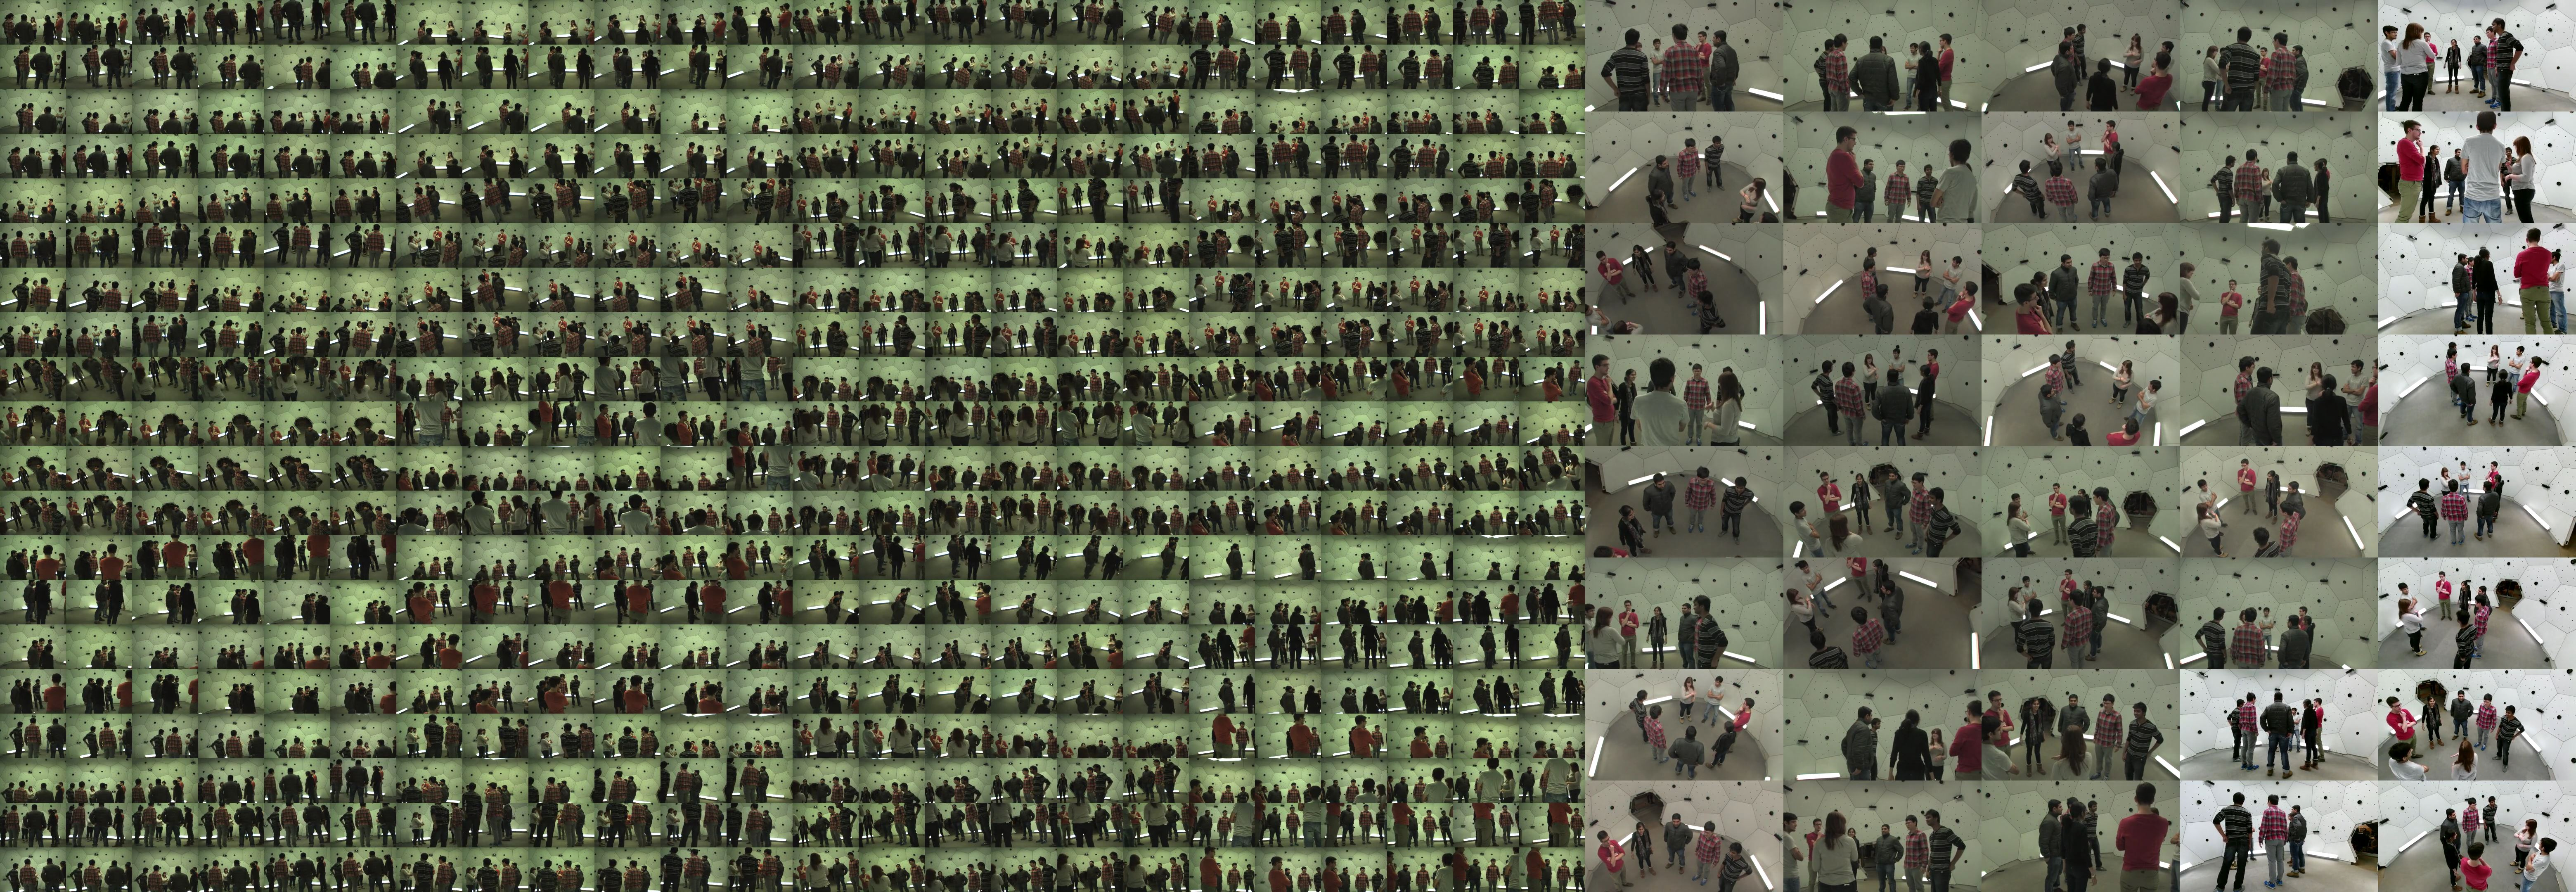
\includegraphics[width=\linewidth]{figures/Teaser}
%		\caption{521 unique views by 480 VGAs, 31 HDs, and 10 RGB+D sensors capturing a social interaction within the Panoptic Studio.} 
%		\label{fig:panopticviews}
%	\end{figure}

%
%\begin{figure}[t]
%	\centering
%	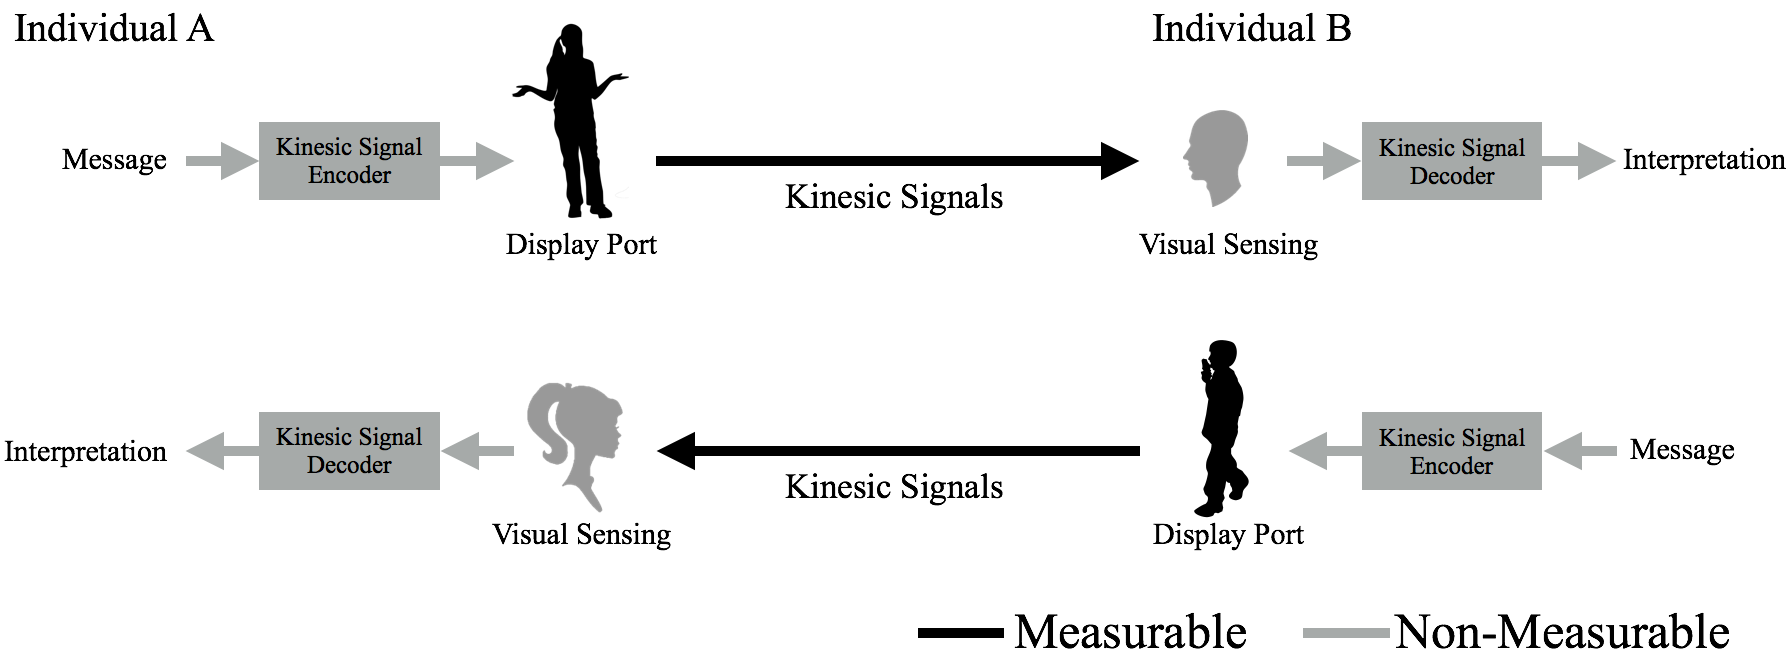
\includegraphics[trim=0 0 0 0, clip=true, width=\textwidth]{figures/kinesicflow2}
%	\caption{Kinesic communication can be considered as an information flow among people. Messages are converted by an encoder and transmitted by our body as a form of kinesic signals. The transmitted signals are sensed, decoded, and finally interpreted by a receiver. We have no clear way to measure the flow or status inside our mind, but only can measure the exposed signals.}	
%	\label{fig:kinesicflow}
%\end{figure}


\begin{figure}[t]
	\centering
	%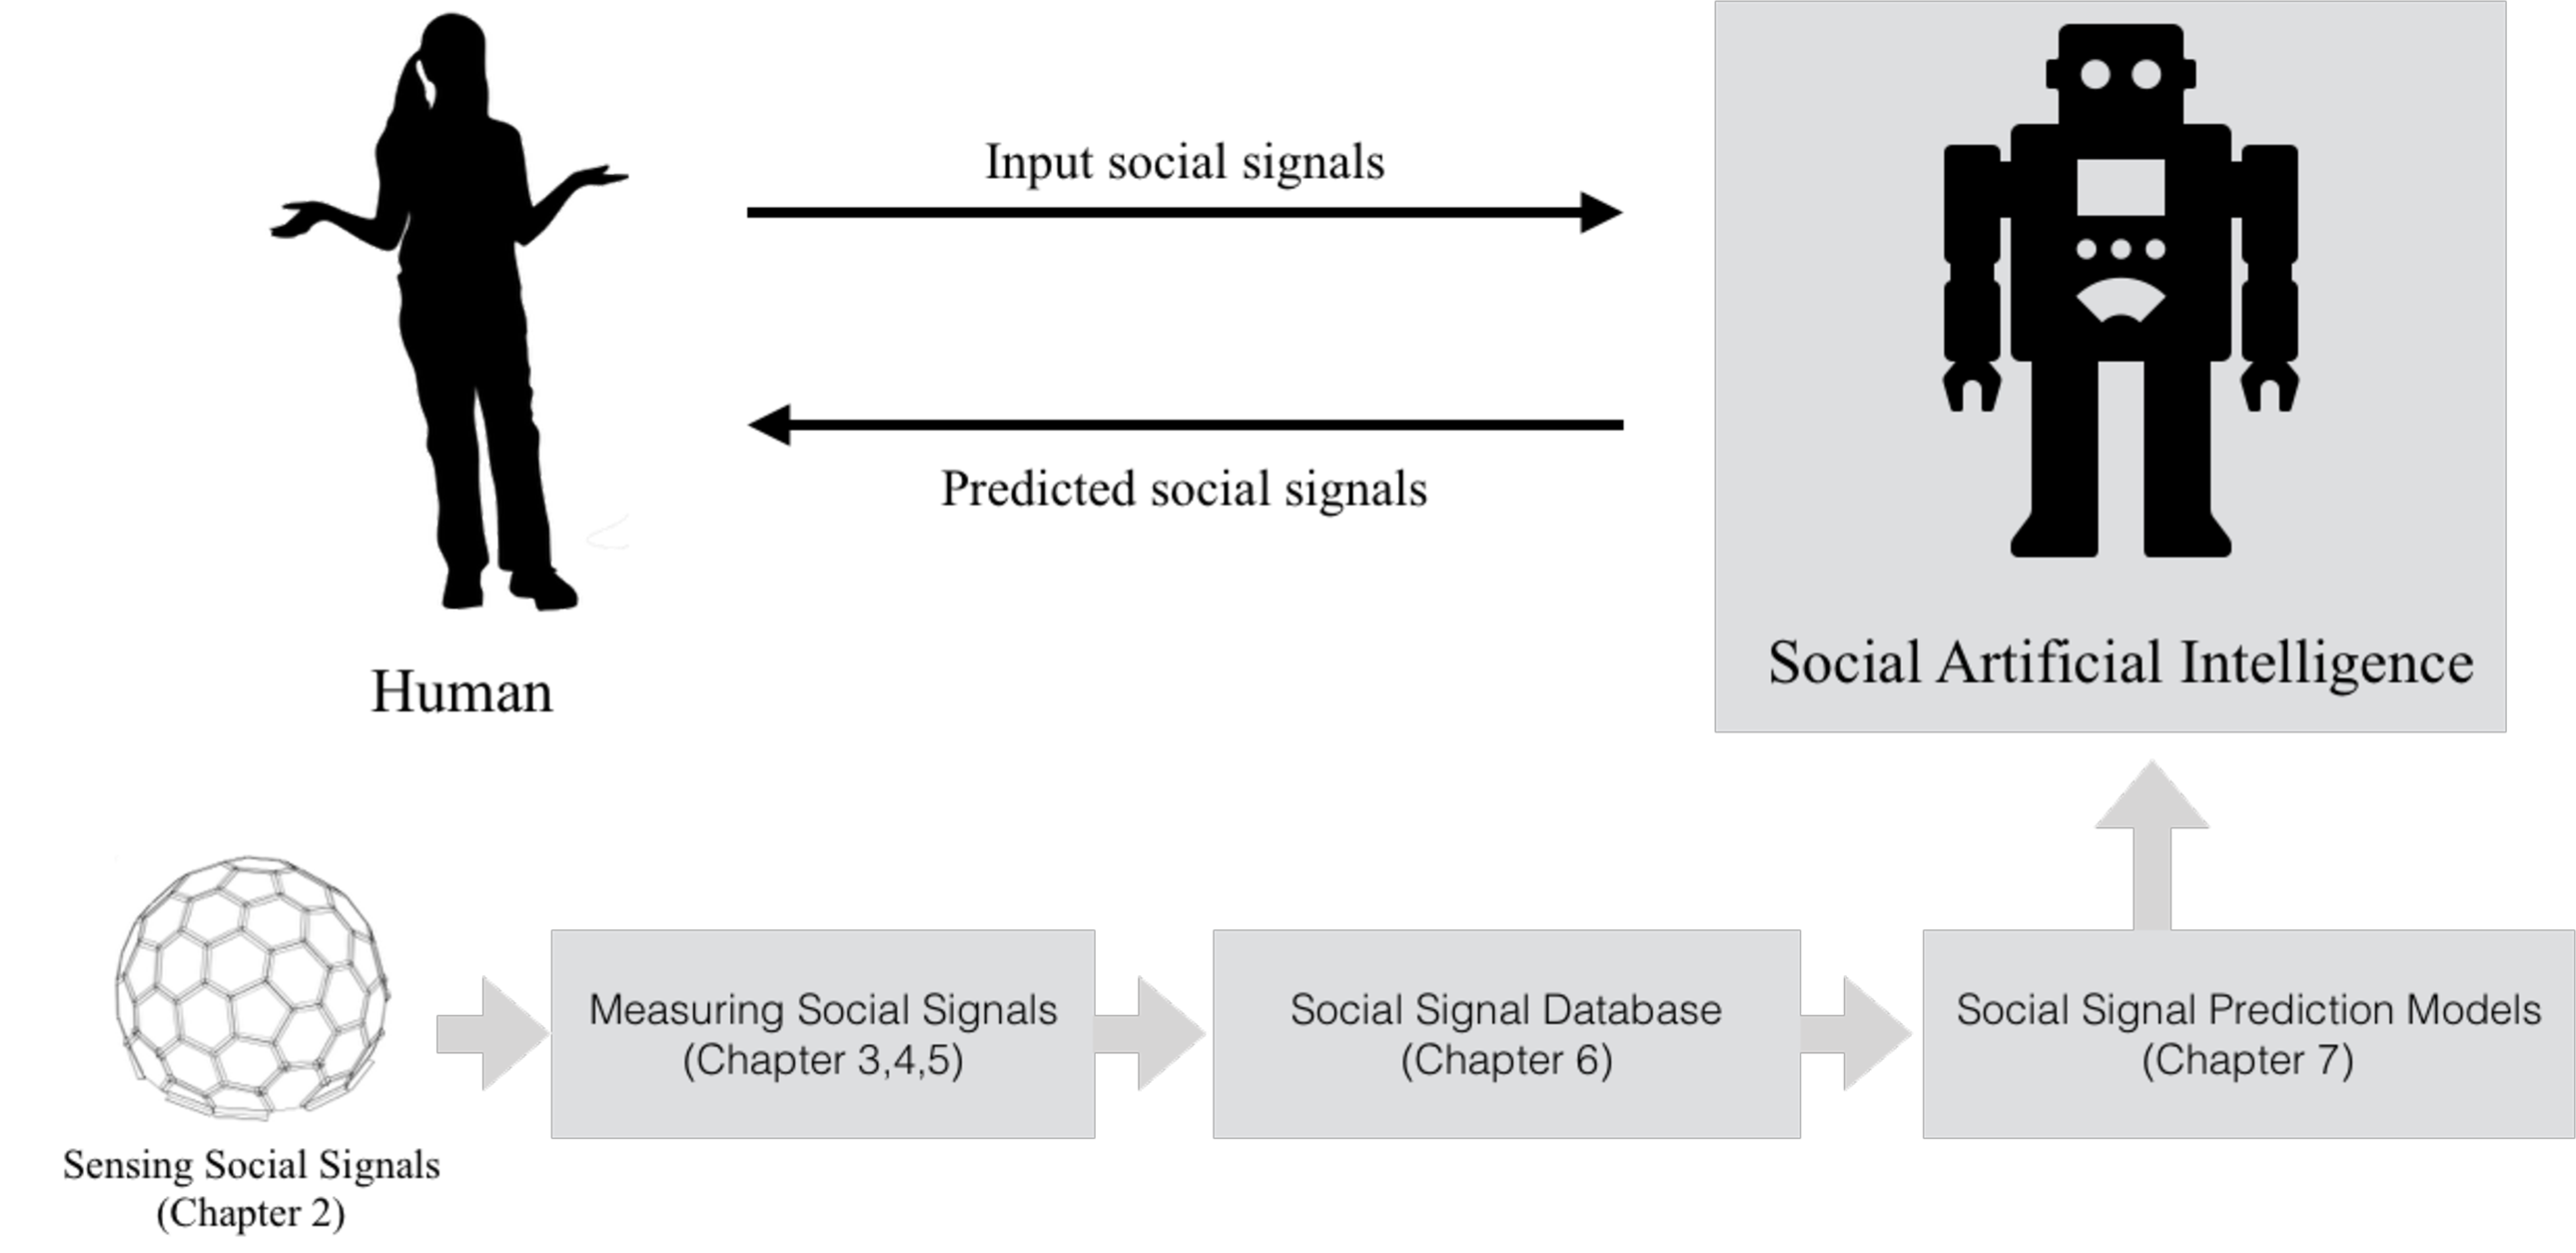
\includegraphics[trim=0 0 0 0, clip=true, width=\textwidth]{figures/intro_framework}
	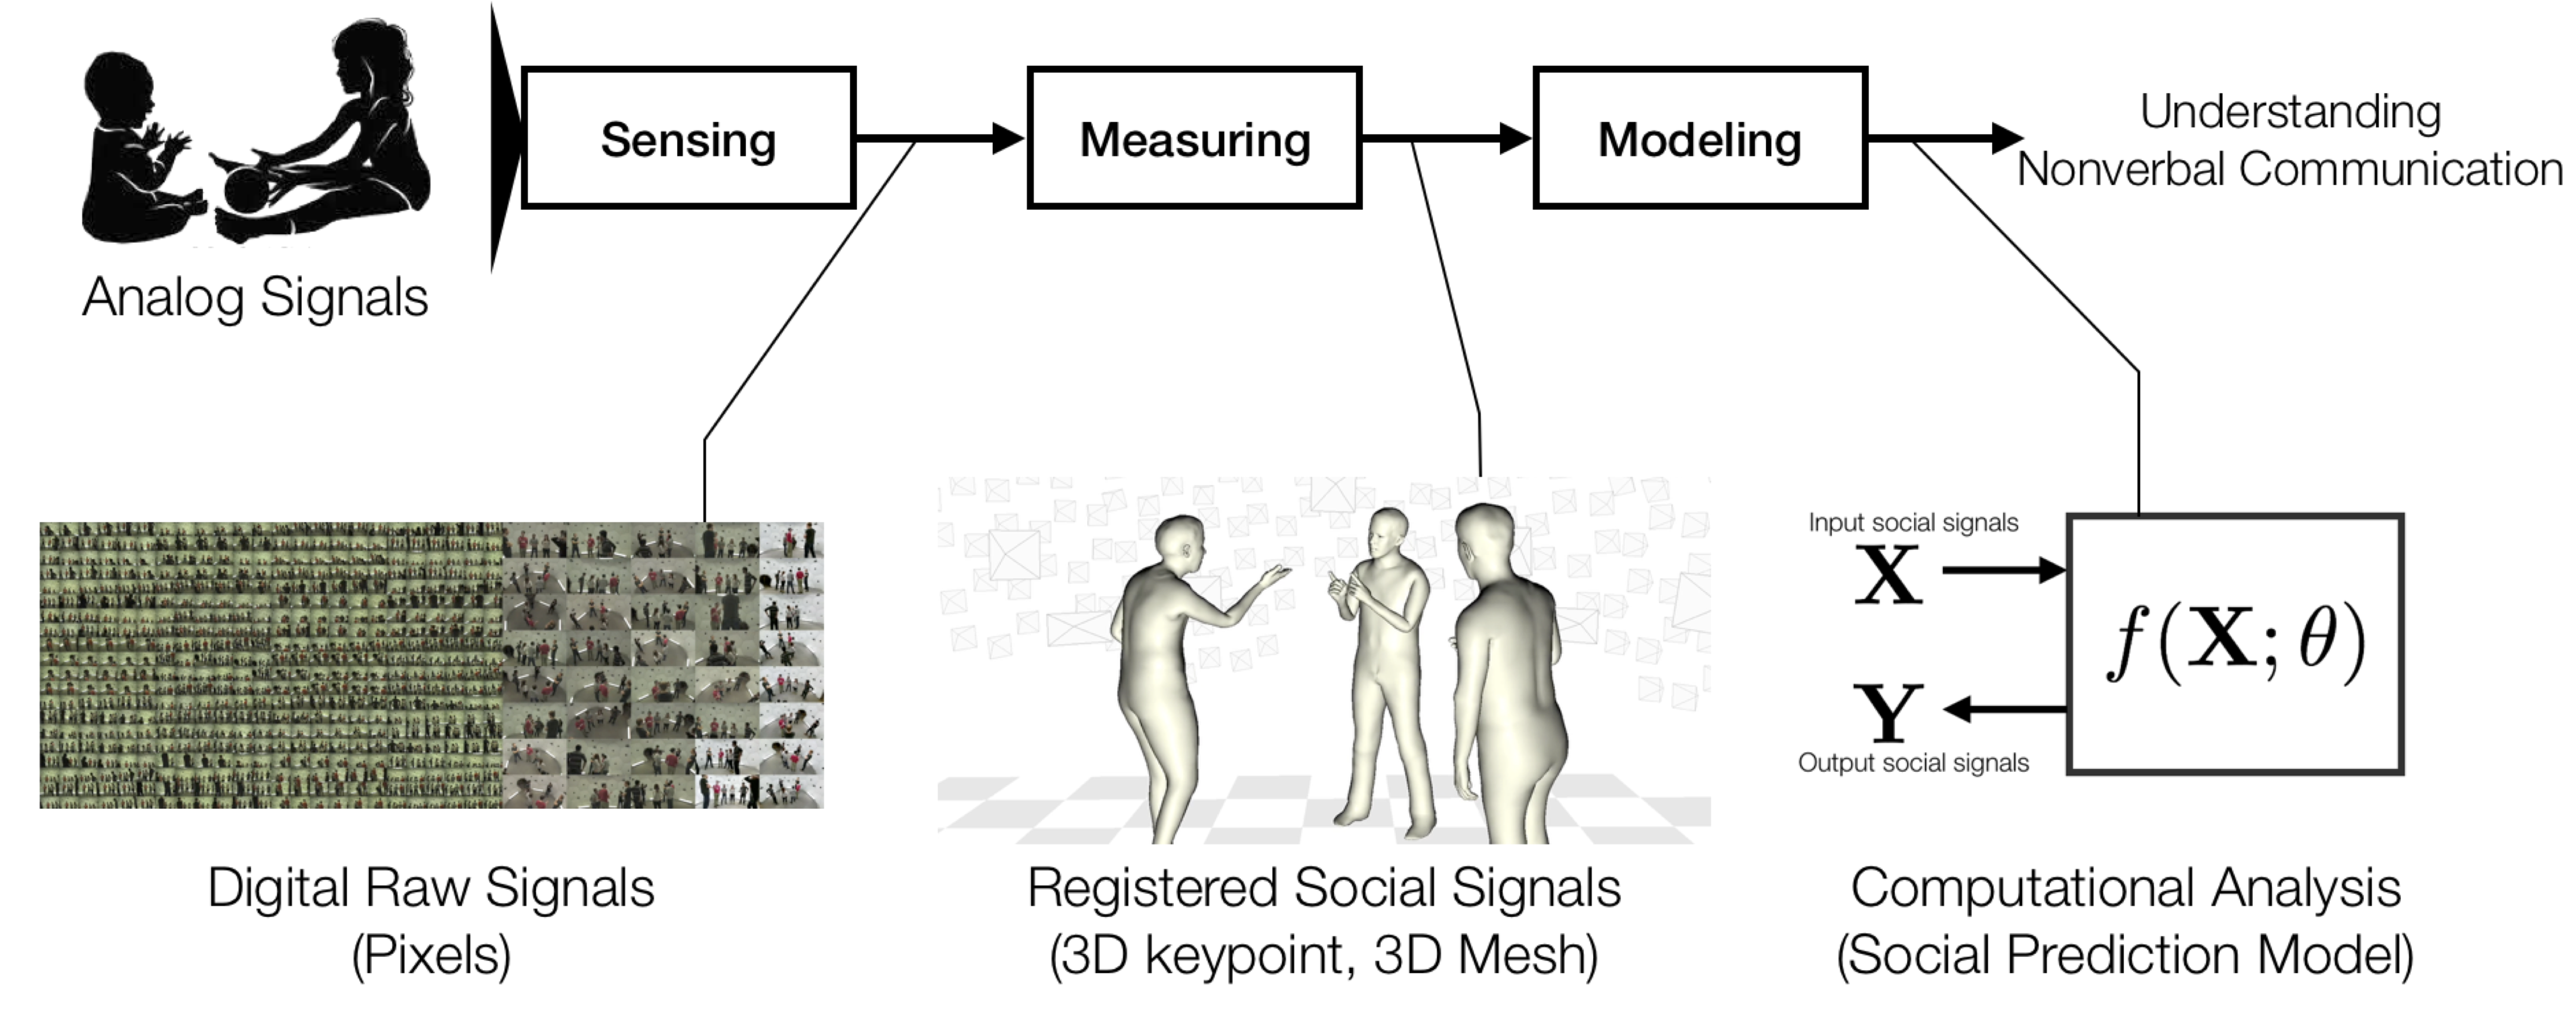
\includegraphics[trim=0 0 0 0, clip=true, width=\textwidth]{figures/overview_threeStages.png}
	\caption{Thesis overview. We explore new approaches in sensing, measuring, and modeling social signals to ultimately endow machines with nonverbal communication abilities}	
	\label{fig:thesis_overview}
\end{figure}



\section{Thesis Contribution}

\noindent \textbf{Thesis statement.}
\emph{We advocate that the full spectrum of social signals---including the body gestures, facial expression, and hand motion---of a naturally interacting group can be measured by a system with a sufficient number of cameras. Based on the measurement, we also argue that such naturally emerging social signals are predictive each other, and modeling their correlation is crucial to enable social Artificial Intelligence.}\\
\mbox{ }\\
\indent This thesis presents a ``full-stack" framework to apply computational methods to model nonverbal social communication. The core contribution of thesis spans a new sensor system to capture interacting multiple people (Chapter~\ref{chapter:system}), a novel methodology to measure the full spectrum of social signals (Chapter~\ref{chapter:trajectory}, \ref{chapter:mocap}, and  \ref{chapter:totalcapture}), a large-scale social interaction dataset (Chapter~\ref{chapter:dataset}), and formalizing a predictive model of social signals (Chapter~\ref{chapter:prediction}). The core contributions of this thesis are summarized below and the an overview of this thesis is illustrated in Figure~\ref{fig:thesis_overview}.
%
%creation of a new scientific discipline of computational behavioral science,
%by measuring the full spectrum of social signals transmitted during interpersonal social interaction.
%
%
%
%The objective of this thesis is to develop a system to measure and model kinesic signals of interacting people. As a core contribution, we build a massively multiview system, the CMU Panoptic Studio, which is composed of 521 heterogeneous camera sensors. Based on the system, we present a method to measure the full spectrum of 3D kinesic signals of interacting multiple people, including the subtle motions of faces, hands, feet, and bodies. Example results are shown in the Figure~\ref{fig:teaser}. A large-scale dataset capturing the interactions of a large number of groups are collected and publicly released\footnote{Panoptic Studio Dataset: \url{http://domedb.perception.cs.cmu.edu/}}.
%
%We also present a framework to model kinesic signals as an information flow among people, by presenting a method to predict kinesic signals of an individual in a social situation. The goal is to build a model to mimic the social communication of humans by producing appropriate response kinesic signals by receiving other people's kinesic signals as input. The model is trained using a Deep Neural Network with a large scale interaction dataset we have collected. We also leverage our social signal prediction model to quantify the amount of information emitted by each body part, which can be interpreted as a way to measure how each channel of kinesic signals contributes in kinesic communication. 

\subsection{Panoptic Studio: A Massively Multiview System (Chapter~\ref{chapter:system})}
We built a new sensor system, the Panoptic Studio, specifically designed to overcome the sensing challenges emerging in social situations. The system is composed of 521 synchronized sensors with different types, including 480 VGA cameras, 31 HD cameras, and 10 RGB+D sensors. The large number of sensors densely cover a large capture volume (5.49$m$ of a diameter) sufficient to have multiple people, enabling to relieve occlusions among interacting people. 

We present a novel modularized design architecture to simplify the complexity of the system. The system is composed of repeated modules with the same shape and architecture, and each module is controlled by a separate local machine. This modularized design makes it easy to control and manage the system, and also enables efficient data acquisition by saving data locally. All cameras are accurately synchronized (or temporally aligned) by a hardware clock, and spatially calibrated in a common 3D world space. The core design choices and technical solutions including structural design, architecture, temporal calibration, and spatial calibration are addressed in Chapter~\ref{chapter:system}.

%, and densely cover the capture volume (5.49$m$ of a diameter) sufficient to have multiple people. The system is composed of three type of sensors: 480 VGA cameras, 31 HD cameras, and 10 RGB+D sensors. The VGA cameras are chosen to have more viewpoints given the same pixel budget, while HD cameras are necessary to capture the detailed structure of body parts such as faces and hands. RGB+D cameras make it easier to obtain a dense 3d point cloud at each time regardless the colors and textures of people. The combination of sensors contribute together in measuring kinesic signals at high resolution including the motion of 3D anatomical landmarks of full body, face, and hands, as well as measuring a dense 3D surface movement. 


\subsection{Measuring 3D Social Signals (Chapters~\ref{chapter:trajectory},~\ref{chapter:mocap},~\ref{chapter:totalcapture})}

We present the first method to measure the full spectrum of 3D social signals including subtle motions from body, face, and hands. The core goals in developing the methods are: (1) simultaneously capturing the \emph{total body motion} of all body parts when a group of people are naturally interacting; (2) building a fully automatic method to capture social sequences at scale without human labor; (3) minimizing assumptions about scenes to be applicable in any type of motion and appearance of arbitrary number of people; and (4) avoiding intrusive approaches, such as attaching artificial markers and avoiding a tedious 3D template building step. To this end, we present a method based on ``weak'' perceptual processes from a large number of views, and robustly measure social signals by satisfying the aforementioned principles. In Chapter~\ref{chapter:trajectory}, a method to reconstruct dense surface movements, which we refer to as a ``trajectory stream", is presented by fusing optical flow cues from the large number of views in 3D. The core challenge of the method is to reason about a time varying visibility to fully exploiting the large number of views. In Chapter~\ref{chapter:mocap}, reconstructing the movement of 3D anatomical landmarks is presented. In this method, we run 2D keypoint detectors for body, face, and hands respectively in each view, and fuse them in 3D to reconstruct 3D locations of anatomical landmarks. By associating them with the trajectory stream, we obtain accurate markerless motion capture results, as well as semantic labeling of the trajectory stream.  In Chapter~\ref{chapter:totalcapture}, we present a novel 3D deformable human body model for total body motion capture, which can express the motions from full body including facial expression and hand gestures in a unified parametric space. 


	
%\noindent \textbf{Proposed Work:} The current measurement results will be spatially and temporally improved by using temporal cues and dense point clouds from multiple RGB-D cameras. Our current method are presented for the goal in this thesis proposal, but it is not able to be applied to long-term sequences of our dataset due to the heavy computational cost. 

%\begin{figure}[t]
%	\centering
%	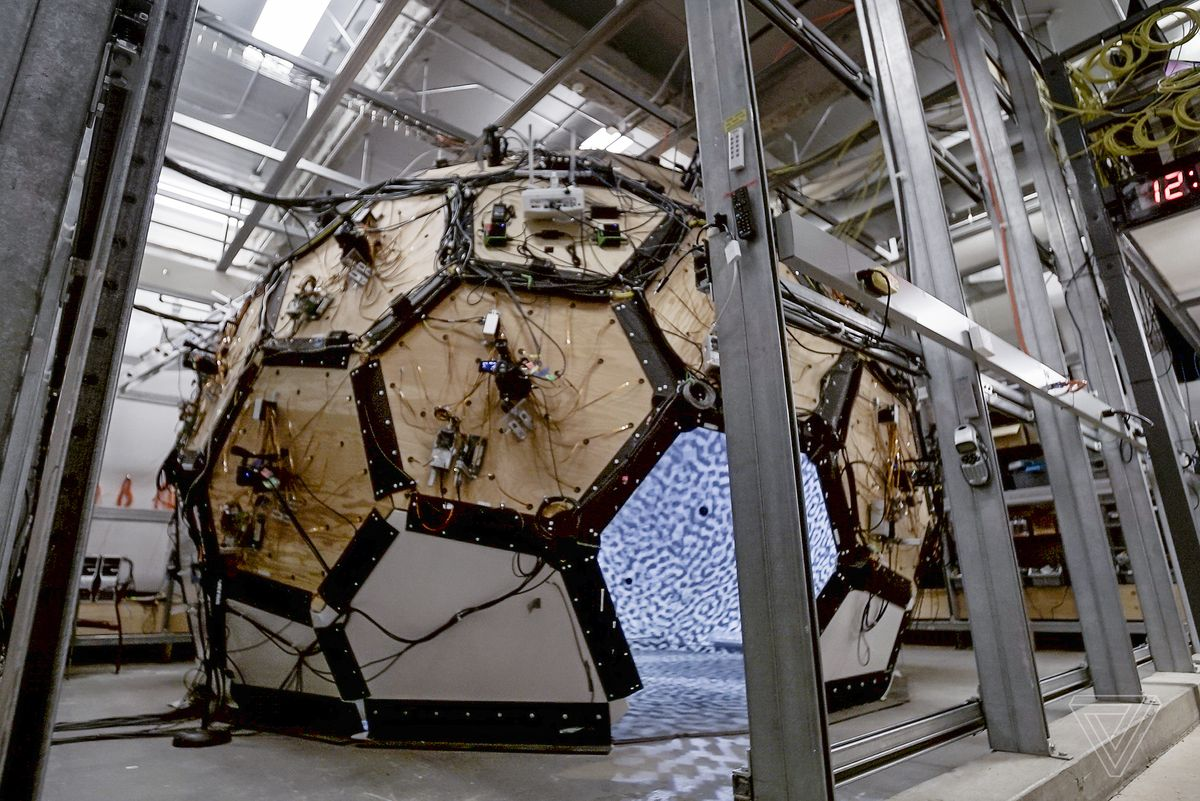
\includegraphics[trim=0 0 0 0, clip=true, width=0.32\textwidth]{figures/panoptic}
%	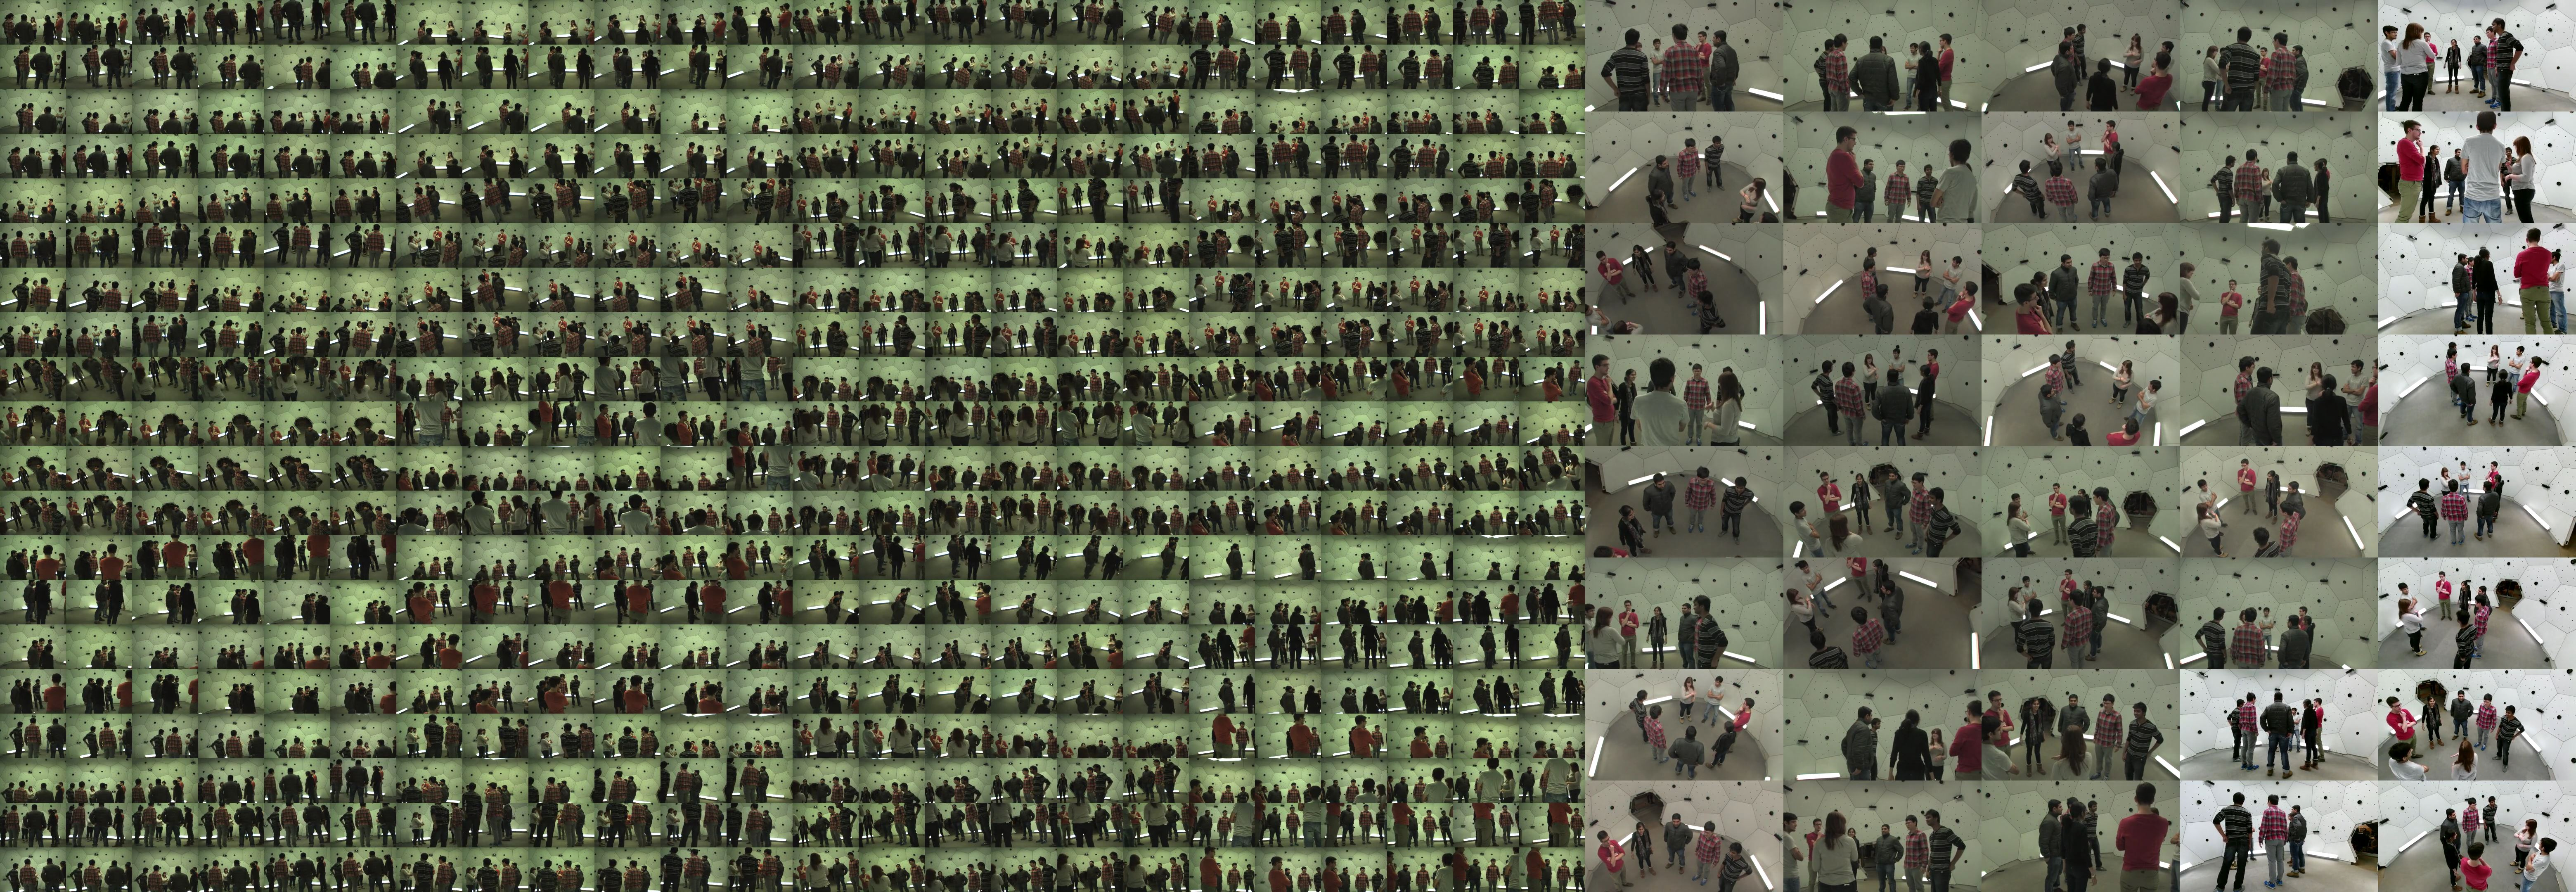
\includegraphics[width=0.62\textwidth]{figures/Teaser}\\
%	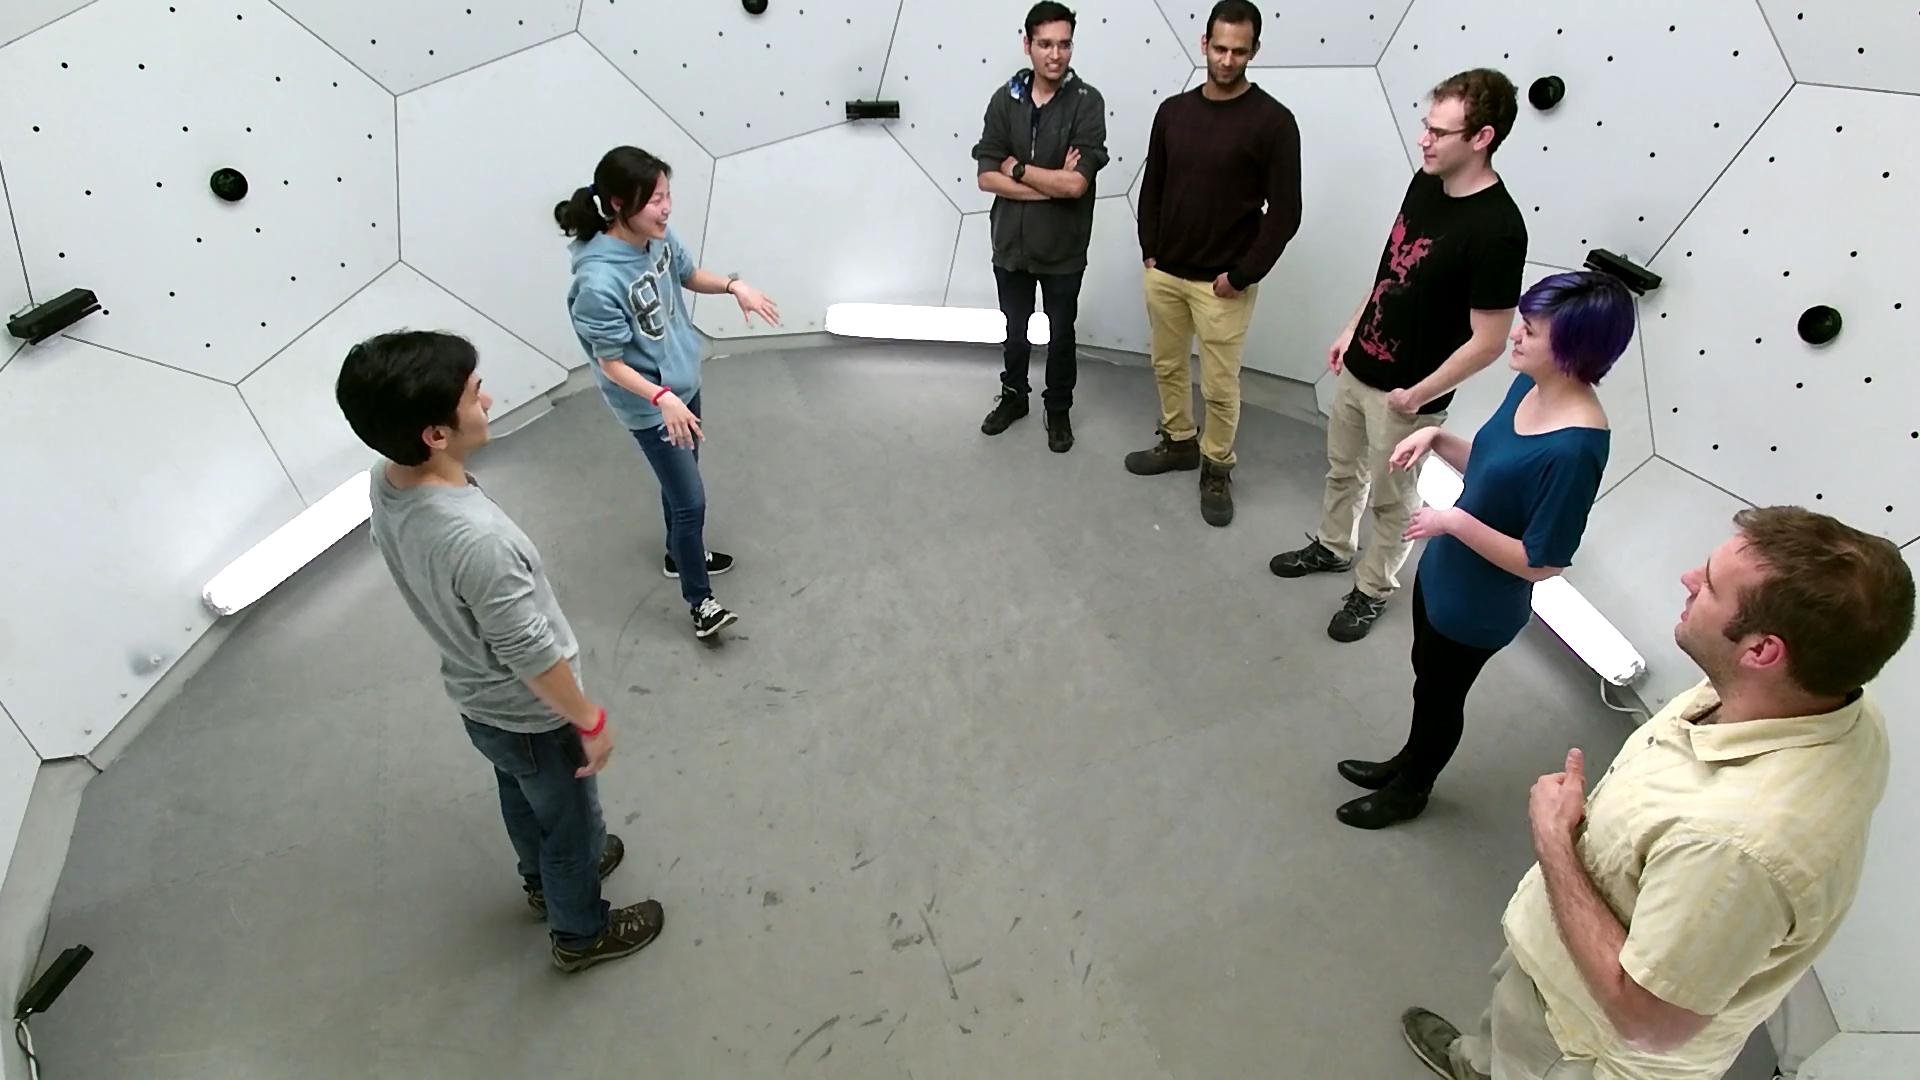
\includegraphics[trim=0 0 0 0, clip=true, width=0.311\textwidth]{figures/teaser_1}
%	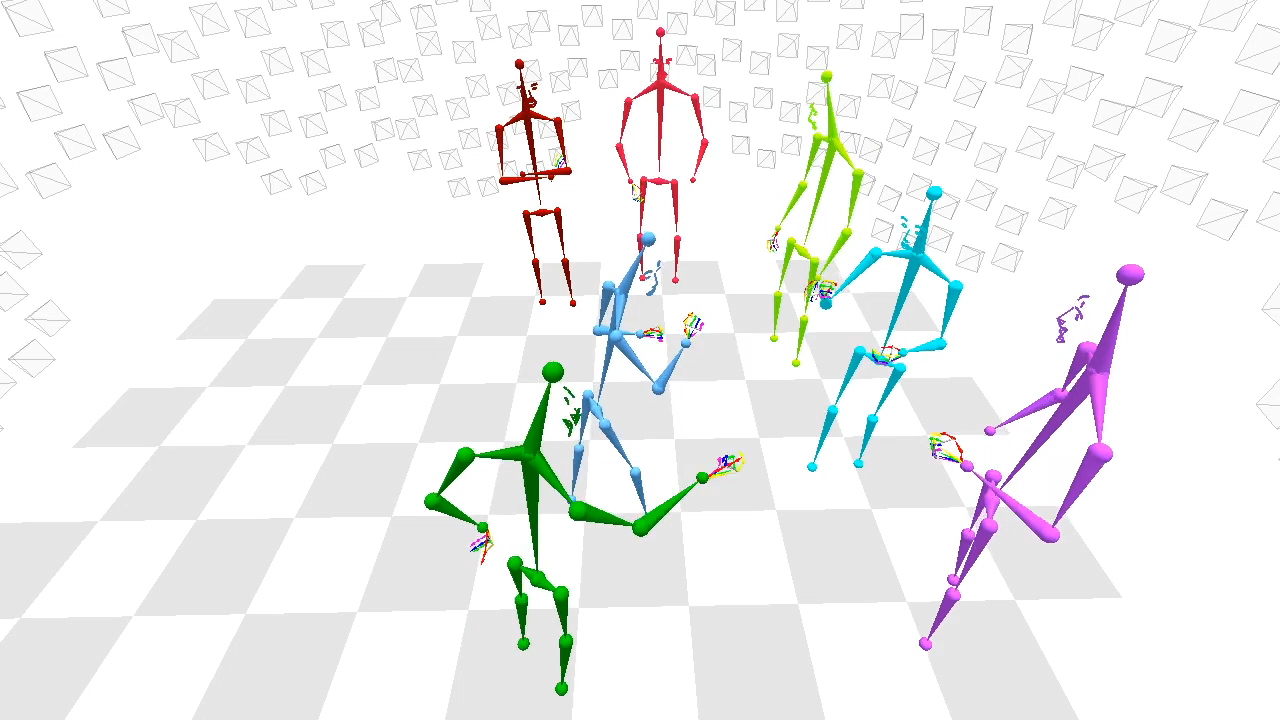
\includegraphics[trim=0 0 0 0, clip=true, width=0.311\textwidth]{figures/teaser_2}
%	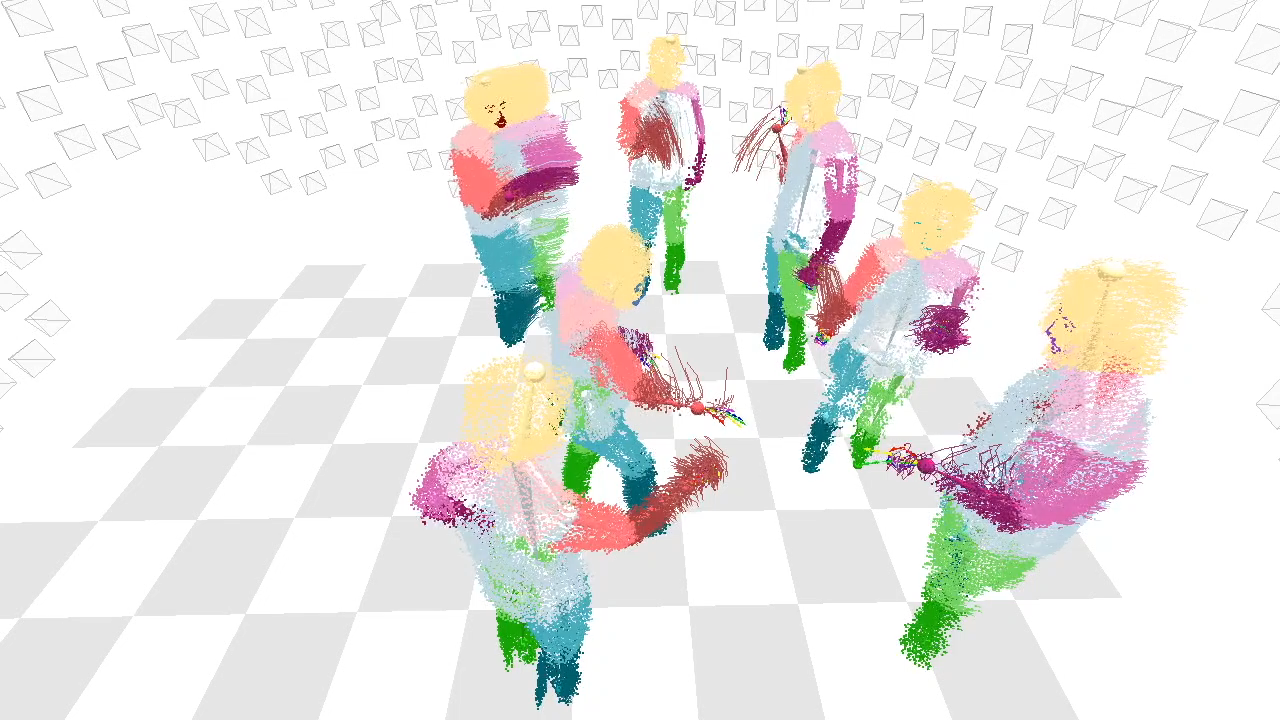
\includegraphics[trim=0 0 0 0, clip=true, width=0.311\textwidth]{figures/teaser_3}
%	\caption{(Top left) The Panoptic Studio, (Top right) 521 unique views by 480 VGAs, 31 HDs, and 10 RGB+D sensors capturing a social interaction within the Panoptic Studio, (Bottom) An example scene captured in the Panoptic Studio and measured kinesic signals.}	
%	\label{fig:teaser}
%\end{figure}


\begin{figure}[t]
	\centering
	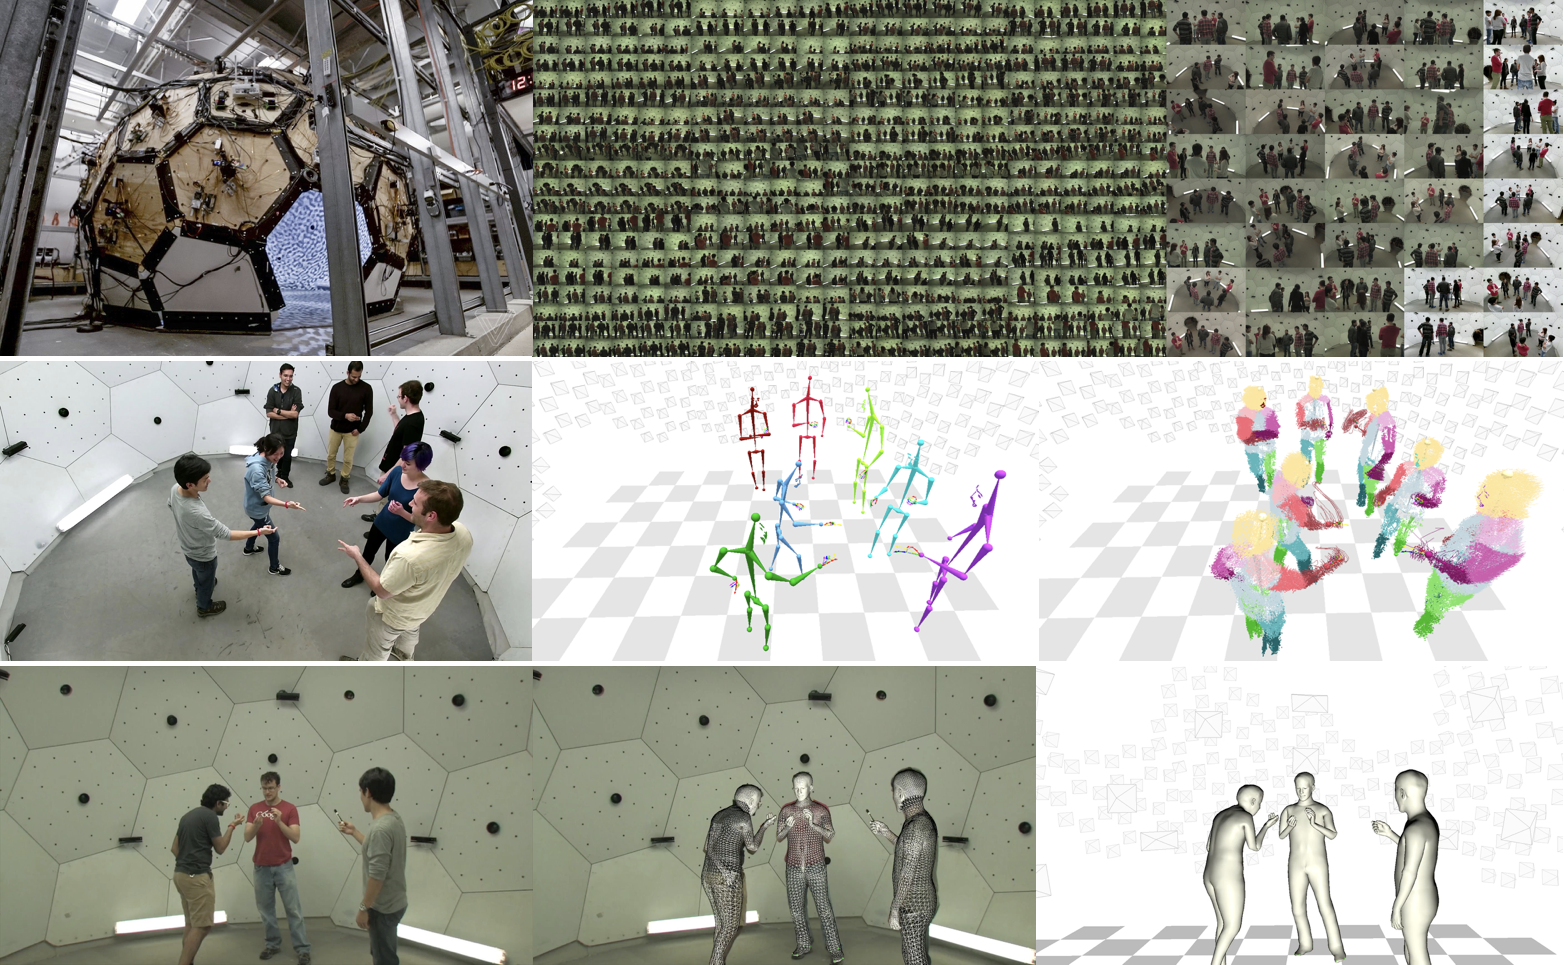
\includegraphics[width=\textwidth]{figures/teaser_4}
	\caption{(Top left) The Panoptic Studio; (Top right) 521 unique views by 480 VGAs, 31 HDs, and 10 RGB+D sensors capturing a social interaction within the Panoptic Studio; (Middle left) An example scene captured in the Panoptic Studio; (Middle center) Measured anatomical landmarks from bodies, faces, and hands; and (Middle right) Measured motion of dense 3D surface points of multiple people; (Bottom) a total motion capture result by the Adam model, showing an input image (left), the reconstruct mesh models overlaid on an input image (middle), and a 3D view (right).}	
	\label{fig:teaser}
\end{figure}

\subsection{A Large-Scale Human Motion Database (Chapter~\ref{chapter:dataset})  }
We build a large-scale dataset by capturing face-to-face interactions of hundreds of participants in our Panoptic Studio. The scenes are captured in a carefully designed triadic negotiation scenario, referred to as \emph{Haggling}, where voluntary social behaviors can naturally emerge. The common social scenario makes it easier to model social interaction, by putting all the subjects in the same social situation. The various behavioral cues including facial expressions, body motions, hand gestures, and individual voices, are sensed and measured by our markerless motion capture system. 

Along with the social game dataset, we also use our system to capture other motions to build a large-scale 3D human motion database. Our database contributes to invent new computer vision techniques. For example, our dataset enables us to build a popular hand keypoint detector~\cite{simon2017hand} in the OpenPose Library~\cite{openpose}, the first deformable 3D human model for total motion capture~\cite{joo2018}, and the first monocular 3D human total capture method applicable in-the-wild~\cite{Xiang2019}. Importantly, we publicly released our dataset in our database website\footnote{\url{http://domedb.perception.cs.cmu.edu}}.

\subsection{Formalizing Social Signal Prediction To Model Nonverbal Interactions  (Chapter~\ref{chapter:prediction})}

We introduce a \emph{Social Signal Prediction} task as a way to computationally model nonverbal interactions. The objective of this task is to predict the behavior of a target person in a social situation. We hypothesize and verify that a target person's behavior is correlated to the behavioral cues of other individuals. For example, the location and orientation of the target person should be strongly affected by the position of conversational partners (known as Proxemics~\cite{Hall66} and F-formation~\cite{kendon90}), and the gaze direction, body gestures, and facial expressions of the target person should also be ``conditioned" by the behaviors of the conversational partners. In this social signal prediction task, we model this conditional distribution among interacting subjects, to ultimately teach a robot how to behave in a similar social situation. In Chapter~\ref{chapter:prediction}, we present several subtasks in modeling a subset of social signals among subject involved in a social interaction, and demonstrate their social signals are predictive. To this end, we present a framework to mimic the nonverbal behavior of the target person responding to other subjects' behavior.%, which we call social Artificial Intelligence. 

%We explore methods to continuously predict high dimensional social signals in social situations based on a data-driven way. Our model takes the social signals emitted by others as input, and produces kinesic signals of the target individual as output. Conceptually, our model regresses a decoder and an encoder in Figure~\ref{fig:kinesicflow} together in a single optimization function, where the decoder interprets the conveyed messages in kinesic signal from others and the encoder transmits the message of target person through kinesic signals. The core advantage of our model is that its input and output are defined by objectively measurable signals, without requiring the representation of the semantic meaning of them. Our model is built using a Deep Neural Network, and trained by the large-scale dataset collected by our Panoptic Studio. Importantly, our model also enables to measure the importance of each body signal in a social communication, quantifying accuracy by eliminating each part signal. The detailed method and preliminary results are presented in Chapter~\ref{chapter:prediction}.


%This thesis demonstrates several state-of-the-art measurement techniques for sensing human behaviors, including the first 3D total body motion capture with a new deformable model~\cite{joo2018}, enabling to build the first 2D hand keypoint detector~\cite{simon2017hand,openpose}, and demonstrating the first monocular 3D total motion capture~\cite{xiang2019}. The system also has been used for many other applications


%the first 2D hand keypoints detector, the first 3D total body motion capture by a new deformable model, and the first monocular 3D total motion capture.


%The new system and measurement method show a broad impact in human sensing fields by demonstrating . 


%gain attentions demonstrate that the full spectrum motion capture is possible to measure the social signals of interacting people. dataset contributes to build a new types of measurement including 3D total body motion capture and hand motion capture and the natrually new potlarge scale system

% This thesis demonstrates several state-of-the-art measurement techniques in computer vision and computer graphics fields, including the first 2D hand keypoints detector, the first 3D total body motion capture by a new deformable model, and the first monocular 3D total motion capture.

%\section{Impact}
%
%This thesis takes an important step to computationally measure and model nonverbal signals to ultimately endow machines with nonverbal communication abilities. The work in this thesis has gained a great attention from the research community. In summary:
%
%\begin{itemize}
%	\item The Panoptic Studio and our markerless motion capture method have been featured on many major media outlets, including the Discovery Channel, Reuters, IEEE Spectrum, BBC News, NBC News, Wired, The Verge, Engadget, and others.
%	
%	\item We organize a tutorial, ``DIY A Multiview Camera System: Panoptic Studio Teardown", in conjunction with CVPR 2017 to share the experience in building multiview systems.  
%	
%	\item Our system is used to build the first 2D hand pose keypoint detector~\cite{simon2017hand}, which is a part of the OpenPose library~\cite{openpose}. The OpenPose library has been selected as a trending repository on GitHub~\footnote{\url{https://github.com/trending/c++}}.
%	
%	%	\item Our system is used for many other applications by artists (Mica, ) and other researchers.
%	
%	\item Our work for total motion capture~\cite{joo2018} won the \textbf{CVPR Best Student Paper Award}, 2018.
%\end{itemize}
%
%The relevant publication list for this thesis is as follows: 
%\begin{itemize}
%	\item  \noindent \href{http://www.cs.cmu.edu/~hanbyulj/14/CVPR_2014_Visibility.pdf}{``MAP Visibility Estimation for Large-Scale Dynamic 3D Reconstruction,"}\\ 
%	Joo et al, CVPR, 2014 \href{https://www.youtube.com/watch?v=LaHTjBWago8}{(Video)}
%	
%	\item \noindent \href{http://www.cs.cmu.edu/~hanbyulj/panoptic-studio/ICCV2015_SMC.pdf}{``Panoptic Studio: A Massively Multiview System for Social Motion Capture,"}\\ 
%	Joo et al, ICCV, 2015 
%	
%	\item \noindent \href{https://ieeexplore.ieee.org/document/8187699}{``Panoptic Studio: A Massively Multiview System for Social Interaction Capture,"}\\ 
%	Joo et al, 2016 (TPAMI 2017 as an extended version of ICCV 2015) \href{https://www.youtube.com/watch?v=m0-7HnWvxG4}{(Video)}
%	
%	\item \noindent \href{https://arxiv.org/abs/1704.07809}{``Hand Keypoint Detection in Single Images using Multiview Bootstrapping ,"}\\ 
%	Simon, Joo, et al, CVPR, 2017 \href{https://www.youtube.com/watch?v=Lajt6vS_dSM}{(Video)}	
%	
%	\item \noindent \href{http://openaccess.thecvf.com/content_cvpr_2018/papers/Joo_Total_Capture_A_CVPR_2018_paper.pdf}{``Total Capture: A 3D Deformation Model for Tracking Faces, Hands, and Bodies,"}\\ 
%	Joo et al, 2018 (CVPR 2018, Best Student Paper Award) \href{https://www.youtube.com/watch?v=5QzdXQSf-oY}{(Video)}	
%	
%	\item \noindent 
%	\href{https://arxiv.org/pdf/1812.01598.pdf}{Monocular Total Capture: Posing Face, Body, and Hands in the Wild"}\\ 
%	Xiang, Joo, et al, 2018
%	
%	\item \noindent 
%	{Towards Social Artificial Intelligence: Nonverbal Social Signal Prediction in A Triadic Interaction"}\\ 
%	Joo et al, 2018
%	
%	\item \noindent Panoptic Studio Database: \url{http://domedb.perception.cs.cmu.edu}
%	
%	
%\end{itemize}



%%%%%%%%%%%%%%%%%% Old intro starts %%%%%%%%%%%%%%%%%% 
%During social communications, we use nonverbal signals to transmit messages and intents that cannot be conveyed with words. For example, it is commonly accepted by social psychologists that much of the emotional meaning is expressed via nonverbal signals \cite{Mehrabian67, Mehrabian81, Birdwhistell70, Moore13}. 
%Nonverbal signals include not only facial expressions and body gestures (also called Kinesics~\cite{Birdwhistell70}), but also all types of ``other-than-words" channels used in communications, including distance between people (e.g., proxemics~\cite{Hall66}), relative position (e.g., F-formation \cite{kendon90}), prosody, physical appearance, haptics, and so on. Interestingly, although we are very familiar with how to use these signals, the underline protocol is still very poorly understood---Sapir~\cite{Sapir-1949} called it ``an elaborate code that is written nowhere, known to no one, and understood by all". Such limited knowledge makes it difficult to transfer the ability of nonverbal communication to machines and robots, and therefore, machines that can convincingly interacting socially with humans do not currently exist. 
%
%Drawing an analogy to telecommunication systems, nonverbal communications also involve senders, receivers, and a ``protocol" to pass messages, where the protocol represents a system of rules to encode and decode the transmitted information via measurable signals. A possible way to decipher the nonverbal code is then by directly modeling the encoder and decoder, based on observed data. For example, happiness and joyfulness can be encoded into a smiling signal expressed by facial muscles. If it were possible to collect a large amount of mappings between the measured nonverbal signals and the transmitted semantic meanings, the protocol could be modeled using a supervised learning technique. In the study of verbal communication, this approach can be applicable. Speech can be transformed (encoded) to languages without ambiguity or losing information. It also follows strict grammatical rules and is composed of well-defined elements, words and phonemes. Once they are transformed into languages they are mostly ready to be further processed to better understand communications.  
%
%
%Much of the nonverbal communication work to date is based on the similar approach (e.g., facial expression database collected by asking subjects to perform a series of predetermined expressions~\cite{de2011facial}), it is comparatively far less understood. The major limitation of this direction is the fact that there is no way to correctly label the messages transmitted via nonverbal signals. The signals are on a continuous space mixed by multiple high dimensional channels, and thus a large amount data is missing if we simply label or describe them by words in discrete levels. Thus, there is no good way to transform the signals to the data to be processed other than saving the signals themselves. 
%
%Three major challenges arise: (1) How to capture social signals; (2) How to measure social signals; and (3) How to understand social signals. First, the social signal can be only captured by observing interacting people in natural scenarios. However, there are principal challenges in capturing social signaling between individuals in a group: (1) social interactions have to be measured over a volume sufficient to house a dynamic social group, yet subtle details of the motion where important social signals are embedded must be captured; (2) strong occlusions emerge functionally in natural social interactions (e.g., people systematically face each other while interacting, bodies are occluded by gesticulating limbs); (3) human appearance and configuration variation is immense; and (4) social signaling is sensitive to interference---for instance, attaching markers to the face or body, a pre-capture model building stage, or even instructing each individual to assume a canonical body pose during an interaction, primes the nature of subsequent interactions. To avoid these obstacles many of previous work restrict the scenarios to a table setup where people are sitting on chairs by limiting their bodily movements~\cite{alameda2016salsa, mccowan2005ami, lepri2012connecting}.
%
%Second, how to measure social signals from recorded videos is not straightforward. To be ideal, stereo images as human does can be used as the input of the system to mimic human's social interaction. However, this basically means that the system should hand all the perception processes as they are performed in humans' brain. Instead, we may consider to extract ``semantic" signals from raw videos, and they including facial expression and body motion, which can be easier to be further processed. However, this also requires to solve multiple fundamental problems in computer vision. 
%
%Third, how to understand the nonverbal communication is largely unexplored area. The major limitation of pursuing such direction is the fact there is no large scale data where model can be trained. Studies to understand human motions are usually based on single person's motion only~\cite{mnih2012conditional, Fragkiadaki_2015_ICCV, jain2016structural}. Otherwise, the previous work is usually based on modeling encoder between the manually annotated labels and coarse signals (which contains the ``biased labeling problem" mentioned above). To be objectively understand the communication, the model should be based on ``observed" signals only which can be measurable by systems.
%
%
%To address these challenges, we develop the ``Panoptic Studio", a novel multiview camera system equipped with 480 VGA cameras, 31 HD cameras, 10 RGB+D cameras, and multiple microphones. This massively multiview system can directly release many capture challenges including covering a large volume, and handling occlusions. There are multiple issues to be carefully considered to design such a big system including synchronization, calibration, capturing system, machine communications, and so on. In this thesis, all the design aspect of the Panoptic Studio is addressed as the results of multiple years of collaboration of several contributors. This paper also address the way to extract various social signals (joint landmarks, facial landmarks, finger landmarks, and dense surface trajectory streams). The core idea in measuring this social signals is based on relatively ``weak" measurement from each view but relying on a large number of views, rather than relying on a complicated template model with strong prior assumption about this scenes. In this thesis, the method and demonstration to measure subtle details of social signals in a fully automatic ways are presented. 
%
%An essential part to understand nonverbal behavior is based on a large scale data. As a core part of this thesis, a large scale dataset is captured and measure using our system. To share the dataset to public, we also build to a system to efficiently share the date to all the research communities. Several aspect in designing the system and dataset is also addressed. More importantly, we scale up the data size in the unprecedented level by inviting hundreds of participants. The game protocol is also carefully designed with a close collaboration psychologists.
%
%As the last chapter of this thesis, we present a method to understand nonverbal communication based on measurable signals. In contrast to the previous work which tries to model the ``encoder" between the message to signal directly, we only use the ``objectively" measurable signal without requiring biased human annotations. To this end, we introduce a novel research problem, \emph{Social Signal Prediction}, problem and study the impact of social signals in predicting future motion of the target humans.  
%%%%%%%%%%%%%%%%%% Old intro ends %%%%%%%%%%%%%%%%%% 
%
%
%\begin{figure}[t]
%	\centering
%	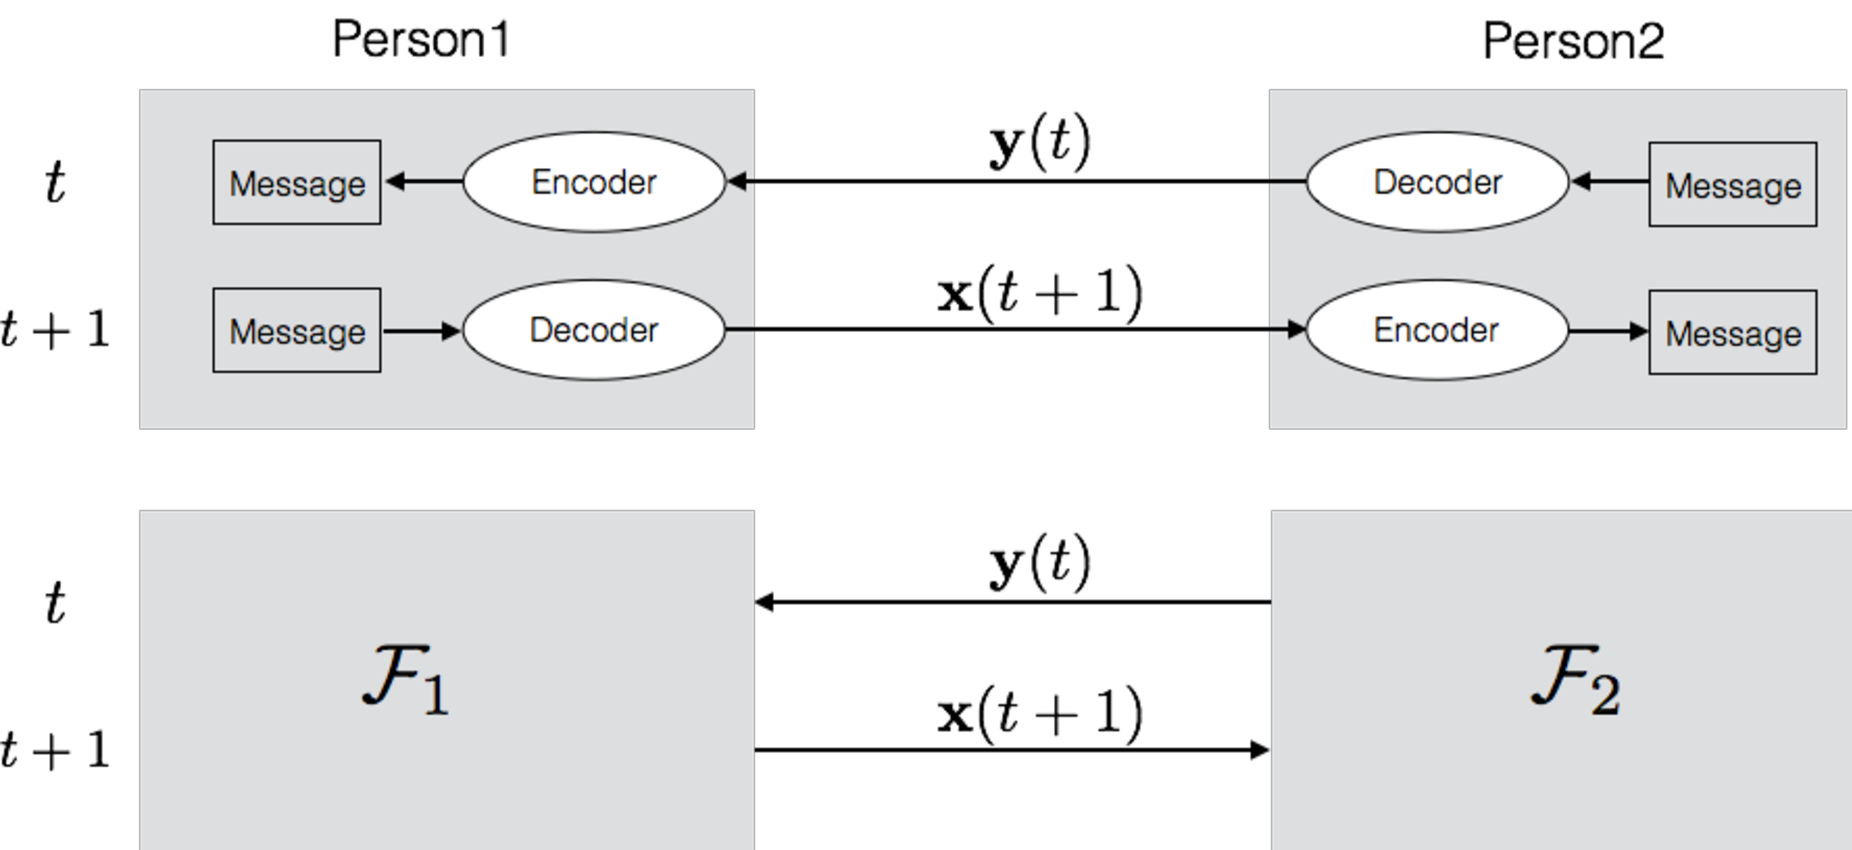
\includegraphics[trim=0 0 0 0, clip=true, width=0.5\columnwidth]{figures/encodDecod2}
%	
%	\caption{Encoder and Decoder model of Social Signals}	
%\end{figure}

%\begin{itemize}
%	\item Motivation: Nonverbal social signals play important role in social communication, transmitting rich information which cannot be conveyed by languages. 
%	\item They are still poorly understood. Why?
%	\item Challenges
%		\subitem - Measurement: large volume, occlusions, immense pose configuration, priming issue (requiring a markerless method).
%		\subitem - Understanding (prediction): high dimensional, hard to model by a hand-crafted way, no available large scale data for ``natural" social interactions, no previous work based on a data-driven method. 
%	\item Our approach
%		\subitem - We present a new capture system and method using massively multiple views: social interaction should be measured by fusing lots of (simple) measurements, rather than complicated methods with a few views
%		\subitem - We present a new data-driven method to model socially interacting multiple people's motion: the model should be trained using a large scale data capturing ``natural" social interactions
%
%\end{itemize}


%\section{Notation}

%During social communication, people use nonverbal body signals using their body movement and facial expression to transmit their intent and emotion. The convey signals have richer information which cannot be conveyed by just using verbal cues. This signal plays very important role, but poorly understood up to now. 

%
%Despite the fundamental role nonverbal cues play in enabling social function~\cite{Birdwhistell-1970,Philpott-1983}, the protocol underlying this communication is poorly understood---Sapir~\cite{Sapir-1949} called it ``an elaborate code that is written nowhere, known to no one, and understood by all". Some structures of this code have been identified through observational study, such as reciprocity~\cite{Brazelton-1974} or synchrony~\cite{Condon-1974}. However, systematic studies of such phenomena have remained almost entirely focused on the analysis of facial expressions, despite emerging evidence~\cite{Meeren-2005,Aviezer-2012} that facial expressions provide a fundamentally \emph{incomplete} characterization of nonverbal communication. One proximal cause for this singular focus on the face is that capturing natural social interaction presents challenges that current state-of-the-art motion capture systems simply cannot address. This paper describes an approach to capture social signals in natural human interactions, presenting fundamental innovations that span capture design architecture, motion reconstruction algorithms, and a large scale dataset capturing more than 3 hours of group interaction scenes using 521 heterogeneous sensors.
%
%There are four principal challenges in capturing social signaling between individuals in a group: (1) social interactions have to be measured over a volume sufficient to house a dynamic social group, yet subtle details of the motion where important social signals are embedded must be captured; (2) strong occlusions emerge functionally in natural social interactions (e.g., people systematically face each other while interacting, bodies are occluded by gesticulating limbs); (3) human appearance and configuration variation is immense; and (4) social signaling is sensitive to interference---for instance, attaching markers to the face or body, a pre-capture model building stage, or even instructing each individual to assume a canonical body pose during an interaction, primes the nature of subsequent interactions. 
%
%In this paper, we present a system designed to address these issues, with integrated innovations in hardware design, motion representation, and motion reconstruction. The organizing principle is that social motion capture should be performed by the consolidation of a large number of ``weak" perceptual processes rather than the analysis of a few sophisticated sensors. The large number of views provide robustness to occlusions, provide precision over the capture space, and facilitate the boosting of weak 2D human pose detectors into a strong 3D skeletal tracker without any prior about the scenes and subjects. In particular, our contributions include: 
%
%	1) \textbf{Modularized Hardware}: We present the modular design of a massively multiview capture consisting of 480 VGA cameras, 31 HD Cameras, and 10 Kinect v2 RGB+D sensors, distributed over the surface of geodesic sphere with a 5.49m diameter (sufficient to house social groups).  %simultaneously triggered/accurate time aligned
%	
%	2) \textbf{3D Motion Reconstruction Algorithm for Interaction Capture}:  We present a method to automatically reconstruct full body motion of interacting multiple people. Our method does not rely on a 3D template model or any subject-specific assumption such as body shape, color, height, and body topology. Yet, our method works robustly in various challenging social interaction scenes of arbitrary number of people, producing temporally coherent time-varying body structures. Furthermore, our method is free from error accumulation and, thus, enables capture of long term group interactions (e.g., more than 10 minutes). 
%	%Our system does not require subjects to: (1) perform any predefined pose for initial alignment; (2) wear clothings with distinctive color from others, (3) directly face sensors to get reasonable measurements; (4) restrict the in-group movement of subjects. All these benefits are key to enabling the study of social interactions at scale. 
%	
%%	3) \textbf{Skeletal Representation}: We present a new representation for social motion capture labeling and embedding a dense 3D trajectory stream within a moving skeletal frame for each individual.
%	%	\item \textbf{3D Motion Reconstruction Algorithm}: We present a novel algorithm, inspired by boosting approaches, for fusing ``weak" human pose detection in each view with 3D tracking, to estimate the articulated nonrigid representation across the diverse set of views
%	%Our algorithm is designed to capture the motion of arbitrary (unknown) number of multiple people, without making prior assumptions about the subjects such as their body shape, texture, and measurement of bone length. Thus, we do not require a predefined model for each individual, or require participants to assume a canonical body pose for initialization during capture. 
%	
%	3) \textbf{Social Interaction Dataset}: We publicly share a novel dataset which is the largest in terms of the number of views (521 views), duration (3+ hours in total), and the number of subjects in the scenes (up to 8 subjects) for full body motion capture. Our dataset is distinctive from the previously presented datasets in that ours captures natural interactions of groups without controlling their behavior and appearance and contains motions with rich social signals as shown in Figure~\ref{fig:iconicPoses} (right). The system described in this paper provides empirical data of unprecedented resolution with the promise of facilitating data-driven exploration of scientific conjectures about the communication code of social behavior. All the data and output are publicly shared on our website\footnote{ \url{https://domedb.perception.cs.cmu.edu}}. 
%	
	
%	
%\section{Proposal Summary}
%\subsection{Completed Work to Data}
%\subsection{Proposed Work}
%\subsection{Timeline}
%\section{Notations}
%
%\section{Multiview System}
%\section{Markerless Motion and Face Capture}
%\section{Social Signal Processing}
%\section{Overview of Contributions}
%\subsection{Timeline}
%\begin{figure}[!ht]
%	\centering
%	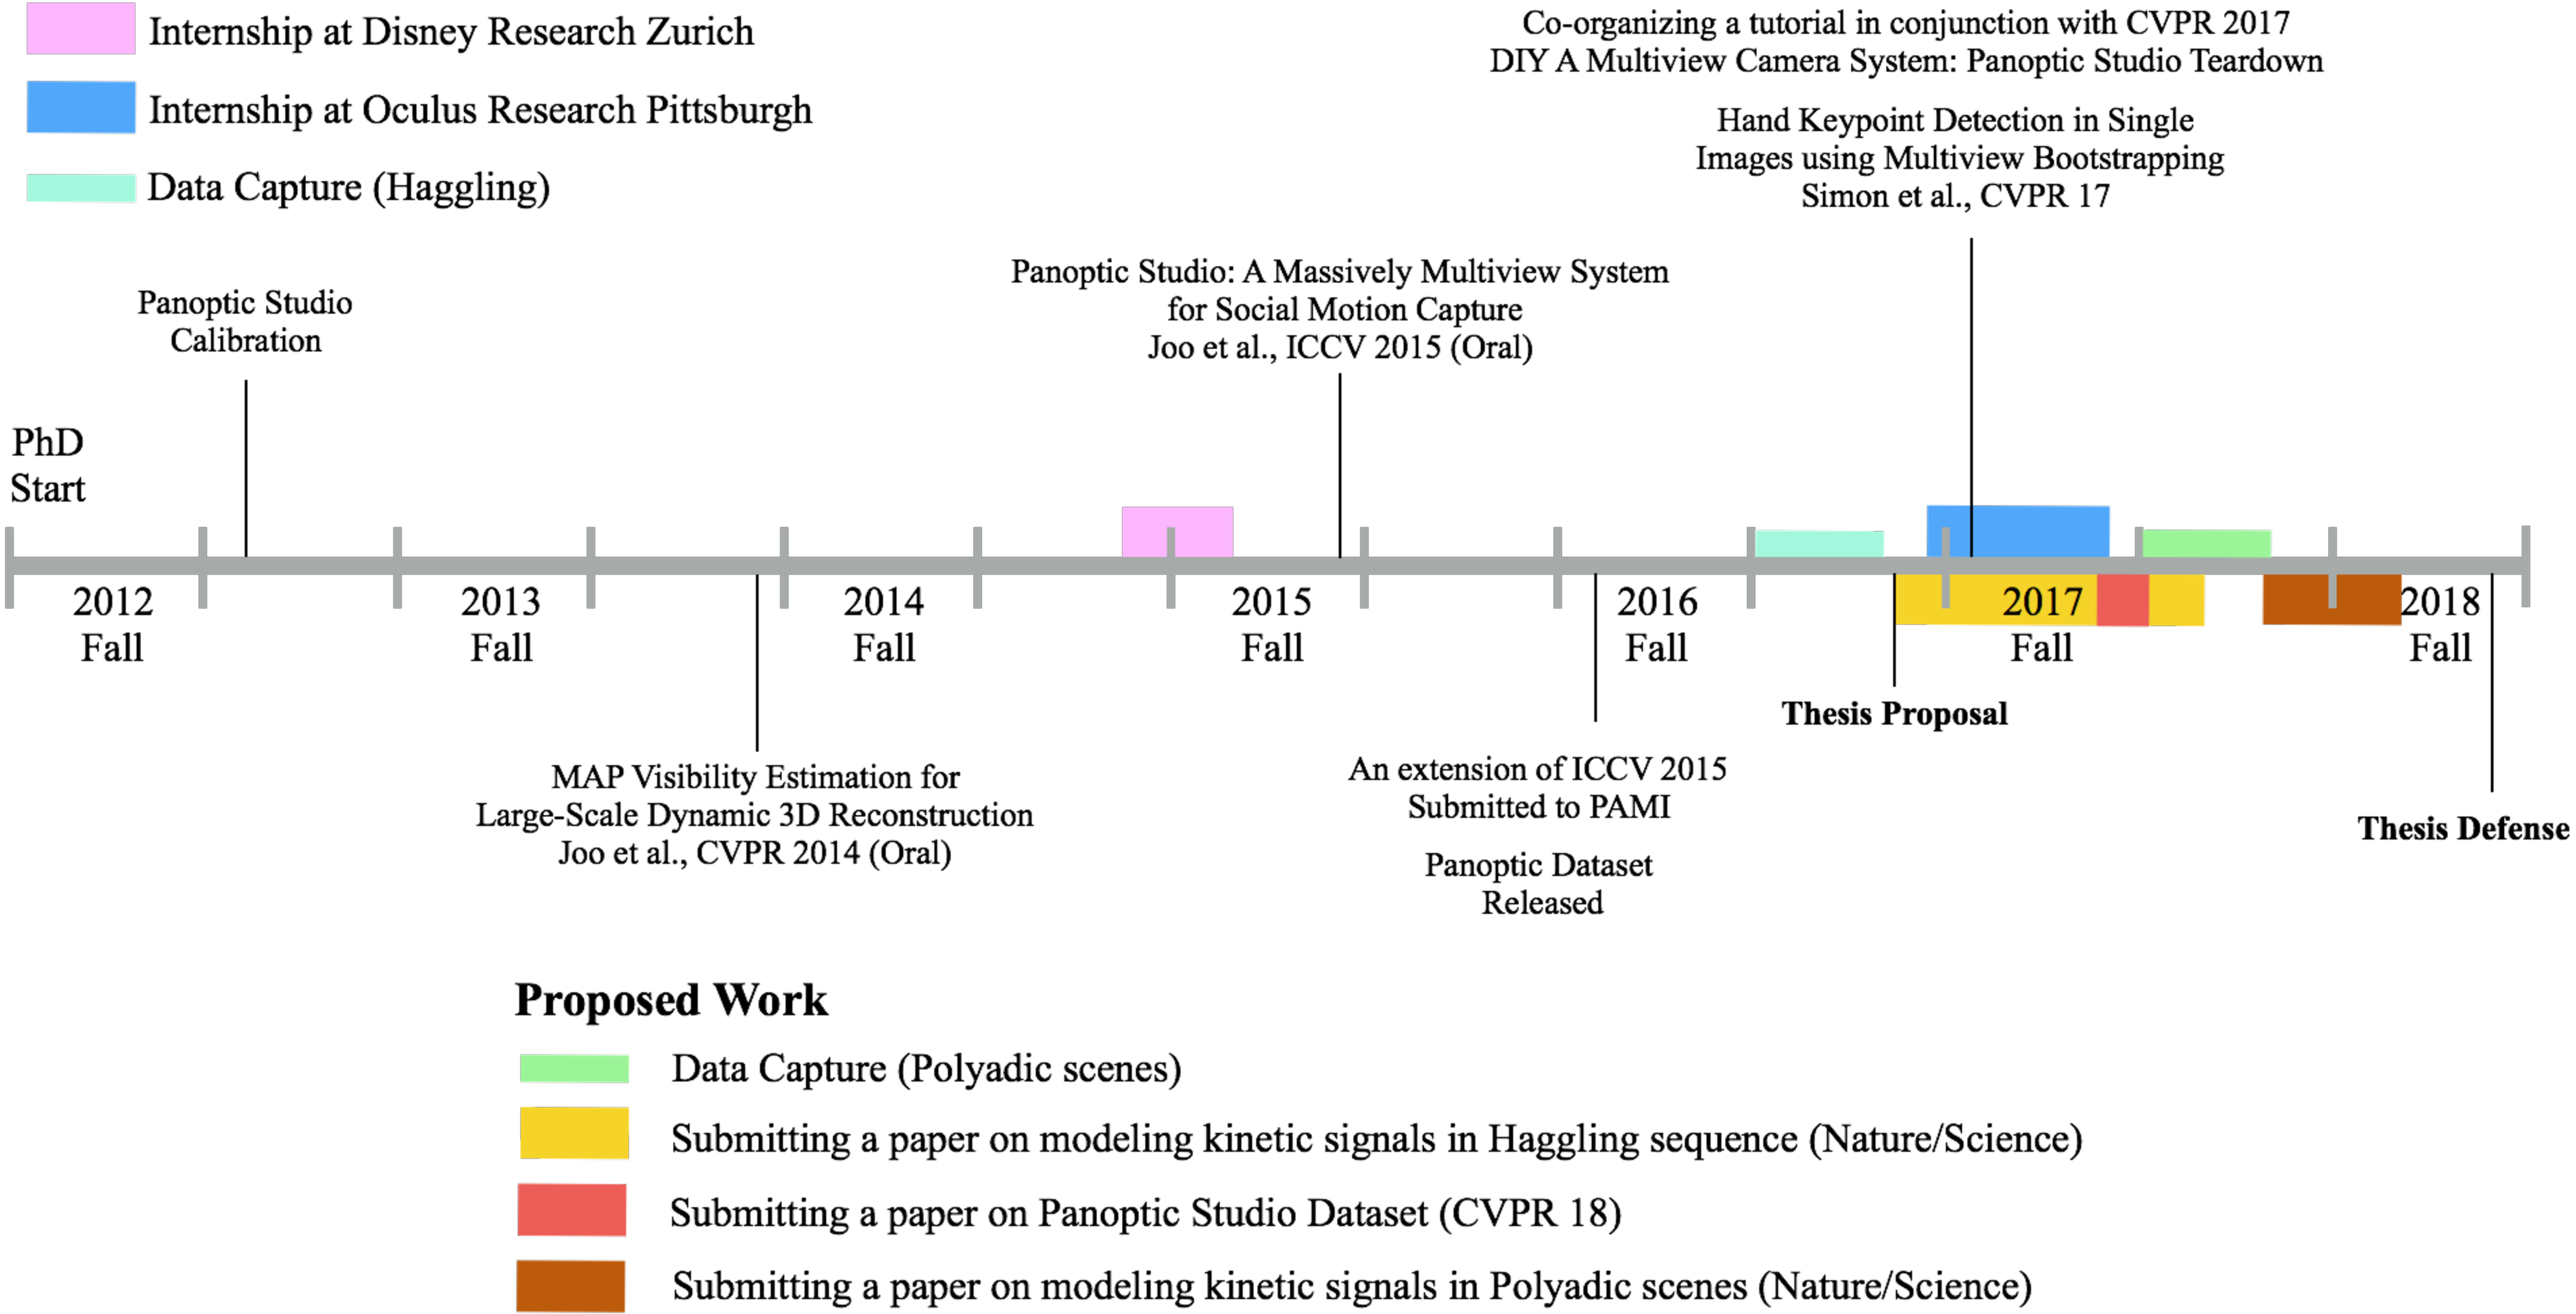
\includegraphics[trim=0 0 0 0, clip=true, width=0.95\textheight,angle=270,origin=c]{figures/timeline}
%%	\caption{A Timeline}	
%	\label{fig:timeline}
%\end{figure}

\newpage 